\chapter{\ehtxt{Numerical} schemes for computing extracellular potentials}
\label{sec:LFPy}
\ghnote{Torbjorn/Espen will write most this.}
\ghnote{La inn forslag til intro her:}

%%%%%%%%%%%%%%%%%%%%%%%%%%%%%%%%%%%%%%%%%%%%%

The established way of computing extracellular potentials is to use a two-step multicompartment + volume conduction (MC+VC) scheme, which can be summarized as:

\begin{itemize}
\item {\bf Step 1:} Compute the electrical activity of neurons using a the multicompartment (MC) framework presented in \Fref{chap:Neuron}, assuming that transmembrane currents are independent on the effect that they have on the extracellular potential ($V_\mathrm{e}$).

\item {\bf Step 2:} Compute the extracellular potential $V_\mathrm{e}$ resulting from the neural transmembrane currents computed in Step 1, using Volume Conductor (VC) theory (\Fref{chap:VC}-\ref{chap:Sigma}).
\end{itemize}

\ghtxt{\sout{
The MC+VC scheme is not self-consistent, since Step 1 computes the neurodynamics under the assumption that $V_\mathrm{e}$ is unaffected by transmembrane currents, while Step 2 uses this neurodynamics to compute a non-zero extracellular potential.} The MC+VC scheme is not self-consistent, since Step 2 computes variations in $V_\mathrm{e}$ due to transmembrane currents, which were computed in Step 1, under the simplifying assumption that they do not affect $V_\mathrm{e}$. Hence, \sntxt{\sout{it} this scheme} does not account \sntxt{\sout{from} for the} feedback-effect from membrane-current induced variations in $V_\mathrm{e}$ on membrane currents.}

\ehnote{I wonder if we should elaborate more on pt. 1: It is entirely possible to impose potentials different from zero and time varying with the current scheme and simultaneously estimate transmembrane currents.} \ghnote{True. I tried to be more precise. }
\ehnote{The main problem is that cable theory is 1D while real neurons are 3D (with the exception of structures such as axonal tracts which may be well approximated as 1D). Self-ephaptic effects should be entirely possible to account for using standard methods (NEURON) for cable models with 1D geometry (at least that's what I think!).} \ghnote{Yes, I think Rall 1977 did this for some 1D cable with an oil-coating, but I do not think this is a relevant model, except under very specific and rare experimental conditions. I think this should be discussed somewhere, but maybe not here?}

There are\sntxt{,} however\sntxt{,} more complete and consistent schemes that account for both the ephaptic effects from $V_\mathrm{e}$  on neurodynamics as well as for effects of ion concentration dynamics on \sntxt{\sout{neuronal activity of}} extracelluar potentials. In general, these more complete schemes require numerical simulations of both the neural and extracellular dynamics using finite element or finite difference methods, and are \sntxt{\sout{very}} computationally expensive.

In most scenarios, ephaptic effects from extracellular potentials on neurodynamics can be assumed to be small, and ion concentrations tend to stay close to baseline. Thus, the simplifying approximations applied in the two-step scheme do not critically affect the accuracy of its predictions. As the MC+VC scheme is far more computationally efficient than any of the more complete schemes, it remains the gold standard for computing extracellular electric signals from large neuronal population models mimicking physiologically realistic scenarios. Also, designated software \sntxt{\sout{has been developed that}} makes it easy to perform simulations using the two-step-procedure. Therefore, the simulations in the application part of this book (Part 2) will predominantly be based on on the MC+VC-framework.

When aiming to make biophysically detailed simulations of extracellular potentials, one might need to simulate large networks containing thousands of neurons. This is computationally demanding, even on an efficient scheme like MC+VC.
\ehnote{Computational demands are linearly dependent on the total number of compartments, so this a "simple" problem to solve, just scale up your computer capability accordingly. Tuning your model with billions of parameters into a reasonable regime is a bigger problem.} As we showed in \Fref{chap:VC}, VC theory provides linear analytical expressions for $V_\mathrm{e}$  as a direct function of the neural current sources (Step 2), meaning that it is usually the simulations of the neurodynamics (Step 1) which is the bottleneck in the simulation. 

We first briefly introduce an alternative, and self-consistent framework (Section \ref{sec:VC:EMI}).
Then, we present computational schemes for the standard MC+VC approach, based on multicompartment neural models (Section \ref{sec:Schemes:LFPy}), and follow up with different strategies that may be applied to reduce the computational cost when computing the neurodynamics using spiking point-neuron models or population-rate models (Sections \ref{sec:Schemes:HybridLFPy}, \ref{sec:Schemes:KernelLFPy}, \ref{sec:Schemes:proxies}). 

\ehnote{For meg gir det mer mening og organisere dette i reduksjonistisk rekkefoelge: (1) self-consistent; (2) MC+VC; (3) point-neuron spiking + MC + VC; (4) firing-rate + MC + VC; (5) Proxies.
Men uansett, burde ikke dette vaere del av "Applications"-kapitlet? Punkt 3 og 4 endrer i prinsippet ingenting med MC+VC formalismen - man disassosierer bare simulering av nettverksaktivitet (korrelasjoner) fra (MC+VC)-formalismen.}


%%%%%%%%%%%%%%%%%%%%%%%%%%%%%%%%%%%%%%%%%%%%%%%%%%%%%%%%%%%%%%%%

\section{\blue{GH: Self-consistent scheme for intra- and extracellular potentials} }
\label{sec:VC:EMI}
\index{Ephaptic effects}

\ehnote{har latt teksten i dette delkapitlet vaere}

Ephaptic effects refers to the phenomenon where the extracellular potential affects the membrane potential dynamics of neurons. The possible importance of ephaptic effects has been the topic of many studies, addressing in various ways how extracellular electric fields may affect neuronal firing or signal propagation in axons (see e.g., \cite**{clark1970,Rall1977,Holt1999,Bokil2001,anastassiou2010,anastassiou2015,Goldwyn2016,capllonch2020,ruffini2020}).

Most of these studies have been based on some simplified approximations as to how evoked fields from one neuron affect other neurons, and less focus has been put on how the presence of ephaptic effects will affect the extracellular potential itself. Rigorous modeling of this, requires that the intra- and extracellular dynamics are modeled simultaneously on a unified framework based on VC theory. Such a framework exists \cite**{Krassowska1994,Agudelo-Toro2013,Tveito2017}, and was in a recent publication referred to as the extracellular-membrane-intracellular (EMI) framework \cite**{Tveito2017}.

\sntxt{\sout{We here only describe very briefly} Here, we briefly describe} the essence of the EMI framework. It is based on (Ohmic) current conservation in the intra- and extracellular spaces, so that:
\begin{equation}
\nabla \cdot \sigma_r \nabla \phi_r = 0,
\label{eq:VC:EMI}
\end{equation}
where $r$ takes the \sntxt{\sout{indexes} indices} $i$ (intracellular space) or $e$ (extracellular space). The intra- and extracellular dynamics are coupled through suitable boundary condictions at the membrane, making sure that a current \textit{entering} the membrane (normal component) at one side of the membrane, is constrained to be identical to the current \textit{leaving} the membrane (negative normal component) on the opposite side \cite**{Krassowska1994}. These entering and leaving currents are in turn determined by a set of mechanisms that jointly determine the transmembrane current $I_m$. In previous numerical implementations of the EMI framework, the membrane currents were modeled with Hodgkin-Huxley like kinetics \cite**{Agudelo-Toro2013,Tveito2017}.

Compared to the two-step MC+VC framework, EMI has the disadvantage that it is computationally expensive. In the MC+VC scheme, which uses volume conduction modeling only for the extracellular space, $\phi_e$ can be computed as an analytical function of the transmembrane neural currents (cf. Chapter \ref{chap:VC}). Using EMI, analytical examples of solutions can only be obtained for idealized scenarios \cite**{Krassowska1994}, while general EMI applications require that both the intra- and extracellular spaces are spatially resolved and their dynamics computed on a numerical framework \cite**{Agudelo-Toro2013,Tveito2017}.

Using EMI to simulate larger systems with realistic morphologies would probably exceed the capacity of today's computers. However, EMI has been used to perform a systematic exploration of the inaccuracies induced when ignoring ephaptic effects in a small system of neurons represented with stylized geometries  \cite**{Tveito2017}.

\snnote{starten paa setningen under klang litt rart for meg, men kan vaere det er helt subjektivt. se forslag}
\sntxt{\sout{There exist even more advanced framework than EMI, which,} Even more advanced frameworks can,} in addition to accounting for ephaptic effects, also account for effects of changing ion concentrations. We will talk briefly of this in Chapter \ref{sec:Eldiff}, where we consider electrodiffusive transports in brain tissue.



%%%%%%

\section{\ehnote{}\ehtxt{Forward-model predictions from multicompartment neuron models and networks}}
\label{sec:Schemes:LFPy}
\index{Multicompartment models}

\ghtxt{\sout{Most models aiming to mimic the dynamics of a particular neuron or neural system except the simplest ball and stick like models are too complex to be solved analytically (cf. \Fref{chap:Neuron}).}With the exception of the simplest ball\sntxt{-}and\sntxt{-}stick\sntxt{-}like models, models aiming to mimic the dynamics of a particular neuron or neural system are generally too complex to be solved analytically (cf. \Fref{chap:Neuron}).} Thus the set of partial differential equations (PDEs) \ghtxt{\sout{and initial conditions}} representing voltage- and concentration-dependent ion channels, synapses, plasticity, neuronal geometry etc. of the full model will have to be solved numerically on computers. The numerical solution of geometrically detailed cable models entails a discretization of the geometry into multiple compartments (hence MC), wherein the states of variables and their derivatives are estimated on a temporal grid which may be fixed or irregular. \ghtxt{\sout{While one could utilize general-purpose numerical solvers in order to compute resulting voltage fluctuations, transmembrane currents or axial currents, a more feasible approach is utilization of one of several different software tools tailored for this purpose that have been developed in the past.}While the state variables in such a model could be computed with a general-purpose numerical solver, a more feasible approach is to use previously developed software tools tailored specifically for simulating neurons. } Such software greatly simplif\sntxt{ies} the process of specifying the \ghtxt{\sout{phenomenological or biophysically detailed}} model and choosing the appropriate numerical schemes for solving the resulting set of PDEs. \ghtxt{\sout{Such tools will also by default usually account for one of the main assumptions of standard cable theory, that is, the spatial variation in membrane voltage across the entire morphology can be computed independently of any effect transmembrane currents may have on the extracellular potential immediately outside the compartments (see chapter \Fref{chap:Neuron} for details).}Most of these tools are by default based on the key assumption made in standard cable theory, i.e., the assumption that the spatial variation in membrane voltage across the entire morphology can be computed independently of any effect transmembrane currents may have on the extracellular potential immediately outside the compartments (see chapter \Fref{chap:Neuron} for details).}

The NEURON simulation environment\footnote{\href{https://neuron.yale.edu}{https://neuron.yale.edu}} \cite**{Hines1997} presently remains a prevalent choice for \ghtxt{\sout{empiric-based}data-based} simulations of MC neuron models as it supports both Windows-,linux- and unix-based operating systems including MacOS, and can be used with a GUI or in a programmatic fashion on laptops, desktop computers and in parallel on large-scale high-performance computing (HPC) facilities. NEURON is also utilized as a simulator backend for other higher-level software such as
PyNN\footnote{\href{https://neuralensemble.org/PyNN/}{https://neuralensemble.org/PyNN/}} \cite**{Davison2008},
NetPyne\footnote{\href{http://www.netpyne.org}{http://www.netpyne.org}} \cite**{Dura_Bernal_2019},
BMTK\footnote{\href{https://alleninstitute.github.io/bmtk/}{https://alleninstitute.github.io/bmtk/}} \cite**{Dai2020},
LFPy\footnote{\href{https://lfpy.readthedocs.io}{https://lfpy.readthedocs.io}} \cite**{Linden2014,Hagen2018} etc.
Alternatives to NEURON with partially overlapping feature sets have been developed in the past in form of
MOOSE\footnote{\href{https://moose.ncbs.res.in}{https://moose.ncbs.res.in}} \cite**{Bhalla2008} and
GENESIS\footnote{\href{http://genesis-sim.org}{http://genesis-sim.org}} \cite**{Bower1998},
while software tailored for point-like neuron models such as
Brian\footnote{\href{https://briansimulator.org/}{https://briansimulator.org/}} \cite**{Stimberg2019} recently received support for biophysically detailed MC neuron models.
Another effort \snnote{virket litt random med denne fundingen, men kanskje relevant?:}\sntxt{\sout{receiving funding from the EU Human Brain Project}},
named Arbor\footnote{\href{https://arbor.readthedocs.io}{https://arbor.readthedocs.io}} \cite**{Akar2019},
aims to develop MC neuron simulation software from the ground up in order to fully exploit modern high-performance libraries and next generation hardware in the form of graphical processing units (GPUs) and massively parallel HPC facilities.

\ghnote{Forslag: Det som kommer nedenfor forvirra meg litt. Jeg er jo vant til at vi definerer $I_m$ og $I_a$ som funksjoner av $V_m$ og regner ut $dV_m/dt$ derfra. Nedenfor kommer en problemstilling som gaar ut paa aa regne ut $I_m$ og $I_a$ fra $V_m$, og hva skal jeg med det? Kan vi gi en intro til det vi skal gjennom? Det er vel slik at vi vil regne ut $V_e$ og kan gjore dette enten via aa kjenne $I_m$ eller $I_a$ (som i dipol-triks etc.). Er det slik at man fra mange simuleringer bare faar ut $V_m(t)$ og at det derfor er praktisk aa kunne noeste seg tilbake derfra til hva $I_m$ og $I_a$ var underveis?  Kan vi skrive ut dette, og evt. dele opp beregningen av $I_m$ og $I_a$ i to underkapitler. Alternativene: (1) Vi faar $I_m$ fra simulering og regner ut $V_e$ fra det. (2) Vi faar $V_m$ fra simulering og regner ut $I_m$ fra det, og saa $V_e$ fra $I_m$. (3) Vi faar $V_m$ fra simulering og regner ut $I_a$ fra det, og saa $V_e$ fra $I_a$...}

\subsubsection{Predicting axial and transmembrane currents}
\label{chap:LFPy_Ia_Im}

\ehnote{nye symboler i samsvar med hva vi naa kommer opp med kommer.}

Here, we will refrain from going into details on the inner workings of the above software tools,
but reiterate that both axial currents and transmembrane currents can be estimated if the set of PDEs can be solved numerically for the membrane voltage of the MC neuron model(s).
The membrane voltages of MC neuron models are typically assumed to be `measured' at the center of each compartment.
The axial and transmembrane currents of a non-branching piece of cable is given in continuous form by
%
\begin{eqnarray}
I_\mathrm{a}(x,t) &=& - \frac{1}{r_\mathrm{i}} \frac{\partial V_\mathrm{m}(x, t)}{\partial x} \text{~and} \\
i_\mathrm{m}(x, t) &=& - \frac{\partial I_\mathrm{a} (x, t)}{\partial x} = \frac{1}{r_\mathrm{i}} \frac{\partial^2 V_\mathrm{m}(x,t)}{\partial x^2}~,
\label{eq:LFPy_ia_im_continuous}
\end{eqnarray}
%
where the intracellular resistance per unit length $r_\mathrm{i}=4R_\mathrm{a}/\pi d^2$ can be given with unit \si{\ohm/\metre}.
Here, $R_\mathrm{a}$  and $d$ is the axial resistivity (w. unit \si{\ohm\metre}) and diameter (unit \si{\metre}) of the dendritic cable model, respectively (cf. \Fref{chap:Neuron}).
The unit for axial currents $I_\mathrm{a}(x, t)$ is \si{\ampere},
while the transmembrane current \sntxt{$i_\mathrm{m}(x, t)$} is per unit length (\si{\ampere\per\metre}).
The location $x$ denotes the position along the piece of cable in one dimension (the cable equation is by definition 1D even if the different parts of a neuron may be assigned locations in 3D space). 

For spatially discretized cable models the axial currents can be estimated per-compartment by the central difference approximation as
%
\snnote{ser ut som om det er et fortegn for mye på andre linje, her:}
\begin{eqnarray}
I_\mathrm{a}(x_j, t) &\overset{h>0}{\approx}& - \frac{1}{r_\mathrm{i}} \frac{V_\mathrm{m}(x_j+\frac{h}{2}, t) - V_\mathrm{m}(x_j-\frac{h}{2}, t)}{h} \nonumber \\
		  &\overset{L_j=h}{=}& \sntxt{\sout{-}} \frac{\pi d_j^2}{4 R_\mathrm{a}} \frac{V_\mathrm{m}(x_j - \frac{L_j}{2}, t) - V_\mathrm{m}(x + \frac{L_j}{2}, t)}{L_j} ~.
\label{eq:LFPy_ia_discrete}
\end{eqnarray}
%
Here, $x_j$ denotes midpoint location,
and the discretization constant $h$ is set equal to the compartment length $L_j$.
Its diameter is typically assumed to be constant,
and the cylindrical compartment is a straight along its length axis.
\ehnote{True for NEURON, but not for Arbor which adapts a FDM type scheme in 1D corresponding to electric compartments made up by series of conical frusta.}
Note that it is possible to swap the central difference approximation
by the forward and  backward difference approximation estimating axial currents for each half-compartment respectively as in \cite**{Hagen2018},
but we will not go into further detail here. 
%For the purpose of computing extracellular signals that may arise from axial currents $I_\mathrm{a}$ we will simply assume that they are piecewise constant currents along the axis of each compartment.


\sntxt{\sout{We next} Next, we} outline how the membrane potential can be estimated at the end points of each compartment $x \in \{x_j-L_j/2, x_j+L_j/2\}$,
which may \sntxt{be} connected to none, one or several other end points of other compartments\sntxt{\sout{, when}. Keep in mind that } the neural simulation software returns the midpoint potential $V_\mathrm{m}(x_j, t)$ for every $j \in \{1, \cdots, N \}$ compartment. For terminating compartments (i.e., one or both ends has no connecting compartments and sealed ends) we may define
%
\begin{eqnarray}
V_\mathrm{m}(x_j - L_j/2, t) &\equiv& V_\mathrm{m}(x_j, t)~\mathrm{and/or} \nonumber \\
V_\mathrm{m}(x_j + L_j/2, t) &\equiv& V_\mathrm{m}(x_j, t)~, \nonumber
\end{eqnarray}
%
depending on which end(s) has no electric connections. \ghtxt{\sout(}This step effectively \ghtxt{\sout{utilize}uses} the forward/backward difference approximation to first derivatives but only \ghtxt{\sout{to}in} terminating compartments. If both ends terminate, the axial current will be zero as the voltage is then implicitly assumed to be iso-potential along the compartment axis.\ghtxt{\sout)} \ehnote{saa kanskje jeg introduserer for/backward difference over allikevel da.} \ghnote{Kanskje, men jeg syntes uansett at dette var tydelig og fint. Man trenger ikke aa vite hva forward/backward difference er for aa henge med.}

For a number $N$ \ghtxt{of} child compartments connected \ghtxt{\sout{at}to} the end point \ghtxt{\sout{location}} $(x_j+L_j/2)$ of the parent compartment (\Fref{fig:LFPy_circuits}C) the potential can be computed from the parent- and child-compartment mid-point potentials as \cite**{Hagen2018}

\begin{equation}
V_\mathrm{m}(x_j+L_j/2, t) = \frac{\sum_{n=0}^N V_\mathrm{m}(x_{j+n}, t) / R_{j+n}}{\sum_{n=0}^N 1 / R_{j+n}}~,
\label{eq:LFPy_V_connect_point}
\end{equation}%
where the connecting node to mid point resistances \ghnote{skjoente ikke formuleringen. Where we have introduced the mid-point resistances:?}
%
\begin{eqnarray}
R_{j+n} &=& \frac{2 R_\mathrm{a}L_{j+n}}{\pi d_{j+n}^2} ~.
\end{eqnarray}

\snnote{Enig i at det er litt kjedelig aa skulle begynne aa snakke om node-til-midtpunkt-resistans. kan vi unngaa det paa denne maaten?}
\sntxt{FORSLAG:
\begin{equation}
V_\mathrm{m}(x_j+L_j/2, t) = \frac{\frac{V_\mathrm{m}(x_j, t)}{r_\mathrm{i}^j L_j/2} + \sum_{n=0}^N \frac{V_\mathrm{m}(x_n, t)}{r_\mathrm{i}^n L_n/2}}{\frac{1}{r_\mathrm{i}^j L_j/2} + \sum_{n=0}^N \frac{1}{r_\mathrm{i}^n L_n/2}}~, \nonumber
\label{eq:LFPy_V_connect_point}
\end{equation}%
where $r_\mathrm{i}^n$is the axial resistance of compartment $n$ with length $L_n$.
}
\snnote{Her har jeg latt parent compartment-leddene ($j$) staa for seg selv, for aa slippe aa bruke $j+n$-notasjon. vet ikke om det totalt sett ble noe bedre..}

For child compartments connecting to the mid point of the parent compartment,
the corresponding potential at the branch point seen by any number of child segments is per definition the same as the mid point potential of the parent, that is,
\begin{equation}
V_\mathrm{m}(x_{j+n}-L_{j+n} / 2, t) \equiv V_\mathrm{m}(x_j, t) ~.
\end{equation}

Up to this point, we have provided the basic `machinery' needed \ghtxt{\sout{in order}} to compute the discrete axial currents in a MC neuron model, independently of \ghtxt{\sout{specific and non-specific ion-channel currents, synaptic currents, capacitive currents etc. which may be present in the membrane of biophysically detailed MC neuron models} any membrane currents present in the model}. By our application of the central difference approximation to the first derivative,
it is in these derivations then implicitly assumed that the axial current is approximately constant along the entire length of the compartment, which in turn implies that the the membrane voltage varies approximately linearly with position.
The naive computational neuroscientist should remind her/himself that this assumption is likely to be violated if the spatial discretization chosen for the model neuron(s) is too coarse.

%
Also the transmembrane currents may be estimated on a per-compartment basis in a similar manner using the central difference approximation to the 2nd derivative as
%
\begin{eqnarray}
i_\mathrm{m}(x_j, t) &\overset{h>0}{\approx}& \frac{1}{r_\mathrm{i}} \frac{V_\mathrm{m}(x_j + \frac{h}{2}, t) - V_\mathrm{m}(x_j, t)+ V_\mathrm{m}(x_j - \frac{h}{2}, t)}{h^2 / 4} \nonumber \\
		&\overset{L_j=h}{=}& \frac{\pi d_j^2}{R_\mathrm{a}} \frac{V_\mathrm{m}(x_j + \frac{L_j}{2}, t) - V_\mathrm{m}(x_j, t) + V_\mathrm{m}(x_j - \frac{L_j}{2}, t)}{L_j^2} ~.
\label{eq:LFPy_im_discrete}
\end{eqnarray}

This machinery may appear as a bit of a hurdle to implement \ghtxt{\sout{for the purpose of computing extracellular potentials or magnetic signals}}, but thankfully MC neuron modeling software such as NEURON and Arbor provide native support for computing the transmembrane current (with unit \si{\ampere}) and/or transmembrane current density per surface membrane area (with unit \si{\ampere/\metre^2}) for each compartment. We will typically assume that the transmembrane current density is equal along each constant-diameter cylindrical compartment (which violates our above assumption of constant axial current!). 
\ghnote{Uklart m/ We will typically assume... Menes: Such software typically assumes?}

Dependent on the implementation in the neural simulation software, a more direct measure of the transmembrane currents \ghtxt{\sout{is indeed}can be obtained with} computing the sum over all capacitive currents, specific and non-specific ion-channel currents, synapse currents etc. (cf. \Fref{chap:Neuron}).
%
\snnote{Hva med aa bare fjerne de neste to setningene?}
The current state \ghnote{forstaar ikke hva current state betyr} is\sntxt{,} however\sntxt{,} a bit more dire with regards to predicting axial current per compartment (or half-compartment \cite**{Hagen2018}). For now, we will emphasize that typical \sntxt{\sout{extracellular}} measures of extracellular electric or even magnetic signals can be derived from the transmembrane currents alone.

\begin{figure}[!ht]
\begin{center}
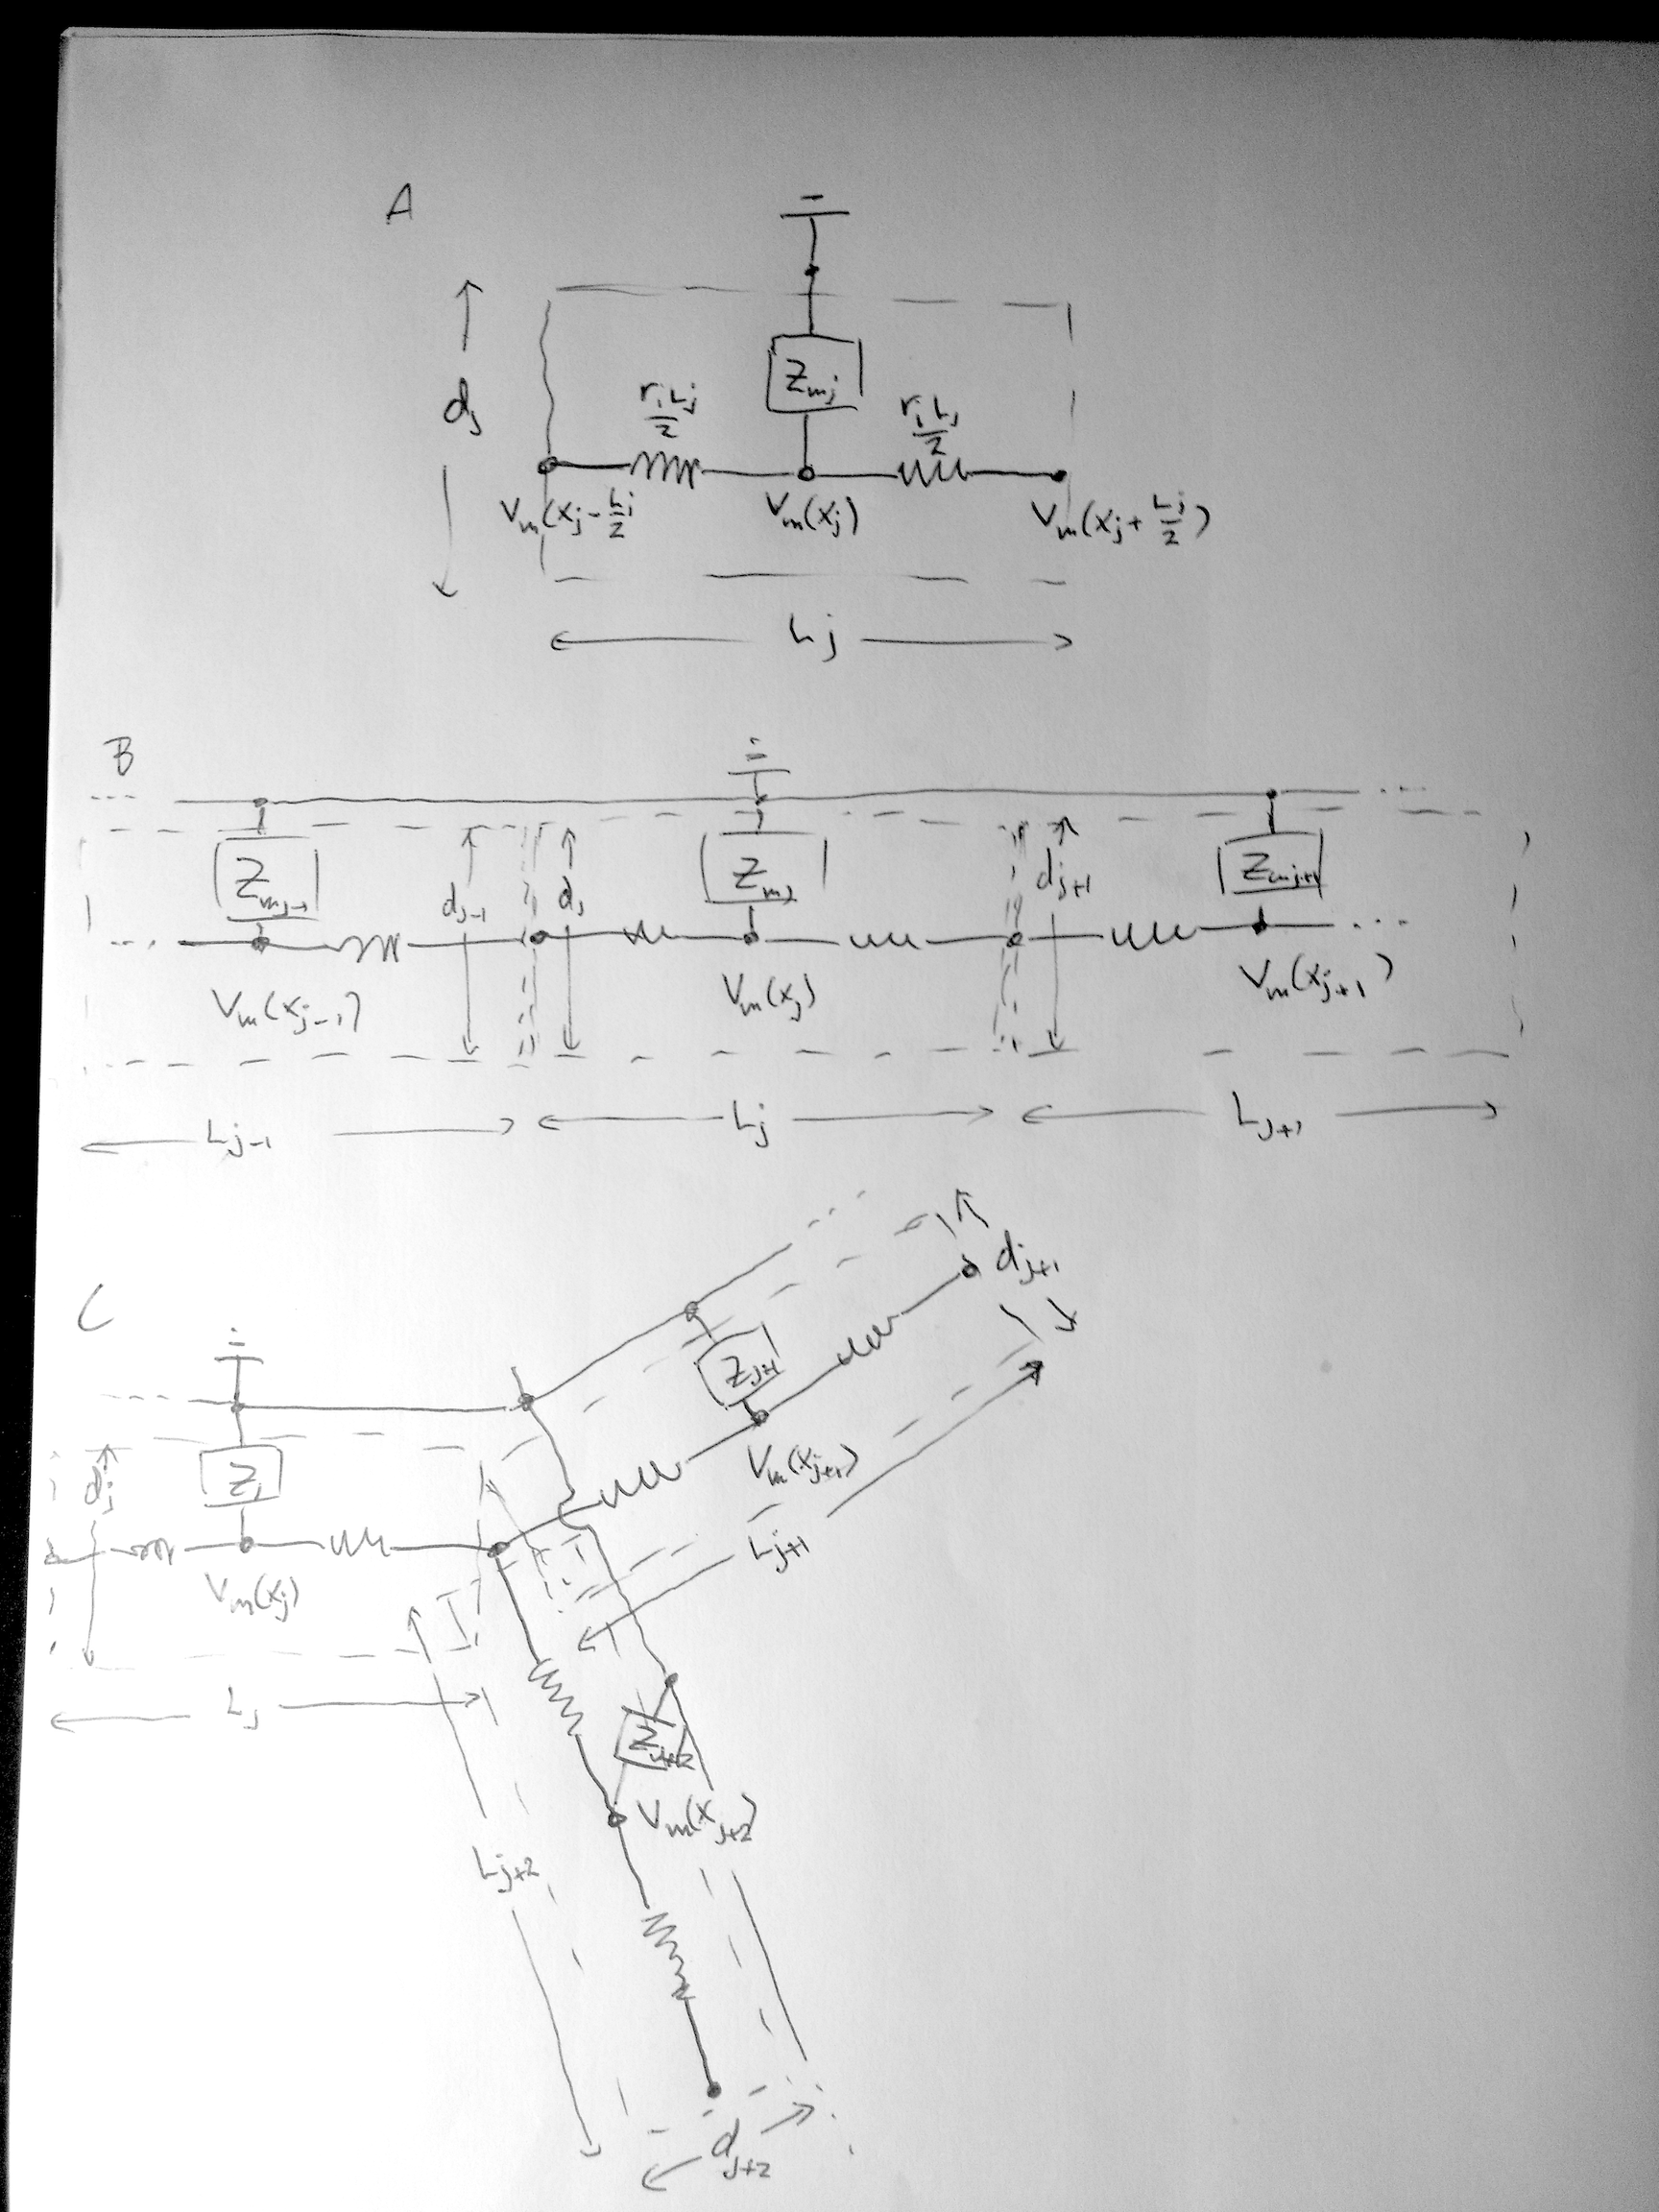
\includegraphics[width=0.8\textwidth]{Figures/Ch-LFPy/circuits.png}
\end{center}
\caption{\textbf{Equivalent circuits for computing axial and transmembrane currents}.
({\bf A}) One-compartment cable model with sealed ends.
({\bf B}) Continuous piece of MC cable model.
({\bf C}) MC cable model with branch point.
\ehnote{ordentlig figur kommer}}
\label{fig:LFPy_circuits}
\end{figure}


Up to this point, the attentive reader of this chapter may have noticed that the axial currents (and transmembrane currents for that matter) is \textit{linearly} dependent on the midpoint membrane voltages of the MC model.
Thus, the full set of operations involved in computing the full set of axial current magnitudes can be rewritten as a linear combination on the form
%
\begin{eqnarray}
\begin{bmatrix}
I_\mathrm{a}(\mathbf{r}_1, t)\\
I_\mathrm{a}(\mathbf{r}_2, t)\\
\vdots \\
I_\mathrm{a}(\mathbf{r}_N, t)
\end{bmatrix}
&=& \mathbf{A}^{-1}
\begin{bmatrix}
V_\mathrm{m}(\mathbf{r}_1, t)\\
V_\mathrm{m}(\mathbf{r}_2, t)\\
\vdots \\
V_\mathrm{m}(\mathbf{r}_N, t)\\
\end{bmatrix} ~,
\label{eq:LFPy_linear_combination}
\end{eqnarray}
%
where $\mathbf{r}_j$ denotes the midpoint location of compartment $j$ while the elements of the shape $(N, N)$ matrix $\mathbf{A}$ effectively corresponds to intracellular resistances and the specific connectivity between compartments
(recall Ohm's law for the current $I$ across a resistor $R$ given a voltage difference $\Delta V$: $I=R^{-1} \Delta V$).
$\mathbf{A}$ may in practise be non-invertible,
but it can be demonstrated that a matrix $\mathbf{G}\equiv \mathbf{A}^{-1}$ can be computed directly.
%
For a two-compartment model connecting the end point of the root (parent) compartment with the start point of the child compartment shown in \Fref{fig:LFPy_circuits}A,
it can be shown with some arithmetics that the axial current in each compartment is \ehnote{derived in /sympycodes/Ch6\_calc\_iaxial.ipynb}
%
\begin{equation}
I_\mathrm{a}(\mathbf{r}_1, t) = I_\mathrm{a}(\mathbf{r}_2, t) =
	- \frac{\pi d_{1}^{2} d_{2}^{2} \left(V_\mathrm{m}(\mathbf{r}_1, t) - V_\mathrm{m}(\mathbf{r}_2, t) \right)}{4 R_{a} \left(L_{1} d_{2}^{2} + L_{2} d_{1}^{2}\right)} ~,
\end{equation}
%
which can be rewritten as the linear combination
%
\begin{eqnarray}
\begin{bmatrix}
I_\mathrm{a}(\mathbf{r}_1, t)\\
I_\mathrm{a}(\mathbf{r}_2, t)
\end{bmatrix}
=
- \frac{\pi d_{1}^{2} d_{2}^{2}}{4 R_{a} \left(L_{1} d_{2}^{2} + L_{2} d_{1}^{2}\right)}
\begin{bmatrix}
1 & -1 \\
1 & -1
\end{bmatrix}
\begin{bmatrix}
V_\mathrm{m}(\mathbf{r}_1, t) \\
V_\mathrm{m}(\mathbf{r}_2, t)
\end{bmatrix} ~,
\end{eqnarray}
%
that is, mathematically similar to \Fref{eq:LFPy_linear_combination}. 
Note that the constant terms have been moved out of the matrix multiplication.
We encourage the interested reader of this book to show that the same approach holds for other model configurations, such
as 3-compartment models without and with branching points as illustrated in \Fref{fig:LFPy_circuits}B and C.

So far\sntxt{,} the axial currents is represented as a scalar field.
For some applications, such as computing the magnetic field $\mathbf{H}(\mathbf{r}, t)$,
the axial currents can be represented as a vector field by multiplication with the path vectors along the center axis of each compartment:
%
\begin{equation}
\mathbb{I}_\mathrm{a}(t) \equiv
\begin{bmatrix}
\mathbf{I}_\mathrm{a}(\mathbf{r}_1, t)\\
\mathbf{I}_\mathrm{a}(\mathbf{r}_2, t)\\
\vdots \\
\mathbf{I}_\mathrm{a}(\mathbf{r}_N, t)
\end{bmatrix}
=
\begin{bmatrix}
I_\mathrm{a}(\mathbf{r}_1, t) \mathbf{d}_1 \\
I_\mathrm{a}(\mathbf{r}_2, t) \mathbf{d}_2 \\
\vdots \\
I_\mathrm{a}(\mathbf{r}_N, t) \mathbf{d}_N
\end{bmatrix} ~,
\end{equation}
%
For compactness\sntxt{,} we introduced the current displacement $\mathbf{d}_j=\mathbf{r}_{\mathrm{f}j} - \mathbf{r}_{\mathrm{i}j}$,
where $\mathbf{r}_{\mathrm{i}j}$ and $\mathbf{r}_{\mathrm{f}j}$ denote\sntxt{\sout{s}} the start- and endpoint coordinates of compartment $j$.
Consistent with the point-source formalism (cf. \Fref{sec:VC:pointsource}),
we let the `location' of each axial current be the mid-point $\mathbf{r}_j$ of each cylindrical compartment $j$.
In a similar manner we will represent the total transmembrane current per compartment as a matrix
\begin{equation}
\mathbf{I}_\mathrm{m}(t) =
\begin{bmatrix}
I_\mathrm{m}(\mathbf{r}_1, t) \\
I_\mathrm{m}(\mathbf{r}_2, t) \\
\vdots \\
I_\mathrm{m}(\mathbf{r}_N, t)
\end{bmatrix}
=
\begin{bmatrix}
i_\mathrm{m}(\mathbf{r}_1, t) \Vert \mathbf{d}_1 \Vert \\
i_\mathrm{m}(\mathbf{r}_2, t) \Vert \mathbf{d}_2 \Vert \\
\vdots \\
i_\mathrm{m}(\mathbf{r}_N, t) \Vert \mathbf{d}_N \Vert
\end{bmatrix} ~,
\end{equation}
under the assumption that the transmembrane current density $i_\mathrm{m}(x_j, t)$ is constant along the compartment axis.
Here, $\Vert\mathbf{d}_j \Vert$ denotes the norm of $\mathbf{d}_j$.
Note that $\mathbb{I}_\mathrm{a}(t)$ is a 3D array with unit \si{\ampere \metre} and shape $(N, 3, N_t)$,
while $\mathbf{I}_\mathrm{m}(t)$ is a 2D matrix with unit \si{A} with shape $(N, N_t)$.
$N_t$ is here the number of discrete time steps in the simulated output signals.


%%%%%%%%%%%

\subsubsection{Application of linear volume conductor models for extracellular potentials and magnetic fields}

As derived from \textit{volume conductor theory} (\Fref{chap:VC}),
the different electric and magnetic signals that can be computed from the electric activity of brain cells are \textit{linearly} dependent on either transmembrane currents or axial currents.
Thus, some arbitrary signals $v(\mathbf{R}_i, t)$ in $M$ different spatial locations from the $N$ compartmental sources located at $r_j$ can be computed as
%
\begin{eqnarray}
\begin{bmatrix}
v(\mathbf{R}_1, t) \\
v(\mathbf{R}_2, t) \\
\vdots \\
v(\mathbf{R}_M, t)
\end{bmatrix}
&=& \mathbf{F}
\begin{bmatrix}
I(\mathbf{r}_1, t) \\
I(\mathbf{r}_2, t) \\
\vdots \\
I(\mathbf{r}_N, t)
\end{bmatrix} ~,
\end{eqnarray}
%
where $\mathbf{F}$ is a matrix with dimensions $(M, N)$ wherein each element $f_{ij}$ is the chosen forward solution mapping the contribution from each source to the corresponding measurement.
For the sake of compactness, $I(\mathbf{r}_j, t)$ is here either represents the axial or transmembrane current of compartment $j$.
A simple linear forward model mapping transmembrane currents of an $N$-compartment model to extracellular potentials in $M$ locations would be the point-source formalism,
which models neuronal sources \textit{and} measurement sites as infinitesimally small points in an infinite homogeneous isotropic and linear volume conductor.
The point-source formula (\Fref{eq:VC:pointsource}) results in elements
%
\begin{equation}
f_{ij} = \frac{1}{4\pi\sigma_\mathrm{e}}\frac{1}{\Vert\mathbf{R}_i - \mathbf{r}_j\Vert}  ~.
\end{equation}
%
The full linear system for obtaining the extracellular potential may then be written out as the linear combination
%
\begin{equation}
\begin{bmatrix}
\phi(\mathbf{R}_1, t) \\
\phi(\mathbf{R}_2, t) \\
\vdots \\
\phi(\mathbf{R}_M, t)
\end{bmatrix}
= \frac{1}{4\pi\sigma_\mathrm{e}}
\begin{bmatrix}
\frac{1}{\Vert\mathbf{R}_1 - \mathbf{r}_1\Vert} & \frac{1}{\Vert\mathbf{R}_1 - \mathbf{r}_2\Vert} & \cdots & \frac{1}{\Vert\mathbf{R}_1 - \mathbf{r}_N\Vert} \\
\frac{1}{\Vert\mathbf{R}_2 - \mathbf{r}_1\Vert} & \frac{1}{\Vert\mathbf{R}_2 - \mathbf{r}_2\Vert} & \cdots & \frac{1}{\Vert\mathbf{R}_2 - \mathbf{r}_N\Vert} \\
\vdots & \vdots & \ddots & \vdots \\
\frac{1}{\Vert\mathbf{R}_M - \mathbf{r}_1\Vert} & \frac{1}{\Vert\mathbf{R}_M - \mathbf{r}_2\Vert} & \cdots & \frac{1}{\Vert\mathbf{R}_M - \mathbf{r}_N\Vert}
\end{bmatrix}
\begin{bmatrix}
I_\mathrm{m}(\mathbf{r}_1, t) \\
I_\mathrm{m}(\mathbf{r}_2, t) \\
\vdots \\
I_\mathrm{m}(\mathbf{r}_N, t)
\end{bmatrix} ~.
\end{equation}
%
Note that the constant terms have been moved out of the matrix multiplication.
Similarly, for line sources (\Fref{eq:VC:linesource}), the elements of $\mathbf{F}$ may be calculated as
%
\begin{equation}
f_{ij} = \frac{1}{4\pi \sigma_\mathrm{e} \Delta s_{ij}} \log \left| \frac{\sqrt{h_{ij}^2+\rho_{ij}^2}-h_{ij}}{\sqrt{\ell_i^2+\rho_{ij}^2}-\ell_{ij}} \right| ~,
\label{eq:LFPy:linesources}
\end{equation}
%
where $\rho_{ij}$ is the distance perpendicular to line segment (compartment) $j$,
$h_{ij}$ the longitudinal distance from the end of the segment
and $\ell_{ij} = \delta s_{ij} + h_{ij}$ the longitudinal distance from the start of the segment to some electrode contact located at $\mathbf{R}_i$.

The approach is applicable also to other types of measurements which are linearly dependent on the transmembrane current sources,
such as the current dipole moment (\Fref{eq:VC:dipole}).
For computing the current dipole moment the mapping matrix' columns are simply
%
\begin{equation}
f_{j} = \mathbf{r}_j
=
\begin{bmatrix}
x_j \\
y_j \\
z_j
\end{bmatrix} ~.
\end{equation}
%
Another example is computing the \textit{ground truth} current source density (CSD) \cite**{Pettersen2008,Hagen2016,Hagen2017},
that is, assigning the contribution of different compartments' transmembrane current to $M$ different volumetric domains $\Omega_i$ as
%
\begin{equation}
f_{ij} = \frac{\Delta s_{ij\in \Omega_i}}{\Delta s_{ij} V_{\Omega_i}} ~,
\label{eq:LFPy:gtCSD}
\end{equation}
%
where $(\Delta s_{ij\in \Omega_i} / \Delta s_{ij}) \in [0, 1]$ denotes the fraction of the length of the segment within the domain $\Omega_i$ and
$V_{\Omega_i}$ the volume of the domain itself.
The geometry of each volume is in principle arbitrary,
however they are typically assumed to be cylindrical or cubic.
Cylindrical volumes can be useful for computing the ground truth CSD alongside a laminar probe \cite**{Pettersen2008,Hagen2016,Hagen2017},
while the latter could be used to compute the ground truth CSD across evenly distributed voxels distributed in the entire 3D space occupied by the neuronal sources.

The formalism using linear combinations may also be adapted for higher-dimensional source elements, that is,
the set of axial currents $\mathbb{I}_\mathrm{a}$ which in the present context can be represented by a 3D array with shape $(M, 3, N_t)$.
\snnote{kanskje bare ta bort "either" i neste setning som den var. eller noe saannt:}
\sntxt{\sout{To compute the magnetic field outside the neuron arising from axial currents one can
either sum up the individual contributions using the relevant Biot-Savart law} \cite**{Blagoev2007,Hagen2018} \sout{as}}
\sntxt{Using the Biot-Savart law, we can compute the magnetic field outside of neurons, by summing up the contributions from axial currents \cite**{Blagoev2007,Hagen2018}:} 
%
\begin{equation}
\mathbf{B}(\mathbf{R}_i, t) = \frac{\mu}{4\pi} \sum_{j=1}^N \frac{\mathbf{I}_\mathrm{a}(\mathbf{r}_j, t) \times (\mathbf{R}_i - \mathbf{r}_j) }{\Vert \mathbf{R}_i - \mathbf{r}_j \Vert^3} ~,
\label{eq:LFPy_biotsavart1}
\end{equation}
%
where the magnetic permeability $\mu \approx \mu_0=4\pi\times 10^7$~\si{\henry/\metre} that is, approximately equal to the permeability in vacuum.
Alternatively,
one can build up a forward model matrix $\mathbf{F}$ element by element as
%
\begin{equation}
f_{ij} = - \frac{1}{4\pi} \frac{I_3 \times (\mathbf{R}_i - \mathbf{r}_j) }{\Vert \mathbf{R}_i - \mathbf{r}_j \Vert^3} ~,
\label{eq:LFPy_biotsavart2}
\end{equation}
%
where $I_3$ is the shape $(3, 3)$ identity matrix,
thus the elements $f_{ij}$ are of shape $(3, 3)$ and $\mathbf{F}$ will be of shape (N, M, 3, 3).
Assuming that each compartmental axial current $\mathbf{I}_\mathrm{a}(\mathbf{r}_j, t)$ is represented as a shape $(3, N_t)$ matrix,
the calculation of the magnetic field $\mathbf{B}$ in location $\mathbf{R}_i$ from all contributions is
%
\begin{equation}
\mathbf{B}(\mathbf{R}_i, t) = \sum_{j=1}^M f_{ij} \cdot \mathbf{I}_\mathrm{a}(\mathbf{r}_j, t) ~.
\label{eq:LFPy_biotsavart3}
\end{equation}
%
Note that application of \Fref{eq:LFPy_biotsavart1} or \Fref{eq:LFPy_biotsavart3} is interchangeable and context dependent.
In situations where axial currents ($I_\mathrm{a}(\mathbf{r}_j, t)$),
current displacement ($\mathbf{d}_j$) and locations ($\mathbf{r}_j$) can be stored separately it may make sense to precompute the full $\mathbf{F}$-matrix for all $M$ measurement sites at once which may demand a lot of system memory.

\ehnote{usikker paa hvor detaljert jeg skal gaa inn her. Python/numpy lar en gjoere en gjoere denne operasjonen for alle maaleposisjoner kompakt som}
\ehtxt{\url{B=(F @ I).sum(axis=1); B.shape=(N,3,Nt); F.shape=(N,M,3,3); I.shape=(M,3,Nt)}}
\ehnote{ogsaa usikker paa notasjon for matriseprodukt med nD matriser som her.}
\snnote{Hadde det holdt aa bytte ut 6.22 med B = F I?}

\subsubsection{Forward models for current dipole moments}
\ehnote{add some on combining current dipole moment to distal measures of activity (EEG, MEG)}
For forward-model predictions of distal electric and magnetic measures of neural activity such as EEG and MEG recordings,
some simplifying steps can be made.
As these signals are measured at distances much greater than the typical extent of the neuronal sources,
the discrete spatial distribution of transmembrane currents $\mathbf{I}_\mathrm{m}(t)$ may be
treated as an equivalent current dipole moment (\Fref{sec:VC:dipole}) defined as the product
\begin{equation}
\mathbf{P}(t) =
\begin{bmatrix}
\mathbf{r}_1 \\
\mathbf{r}_2 \\
\vdots \\
\mathbf{r}_N
\end{bmatrix}
\begin{bmatrix}
I_\mathrm{m}(\mathbf{r}_1, t) \\
I_\mathrm{m}(\mathbf{r}_2, t) \\
\vdots \\
I_\mathrm{m}(\mathbf{r}_N, t)
\end{bmatrix} ~,
\end{equation}
which is equivalent to \Fref{eq:VC:dipole}.
As $\mathbf{r}_j \equiv [x_j, y_j, z_j]^\top$, 
the resulting shape of the current dipole moment array will be $(3, N_t)$.

In the relatively simple case of an infinite homogeneous volume conductor the extracellular potential resulting from the current dipole moment is
\begin{equation}
\phi(\mathbf{R}, t) = \frac{\mathbf{P}(t) \cdot (\mathbf{R-r})}{4 \pi \sigma \Vert \mathbf{R-r} \Vert^3} ~,
\label{eq:LFPy:dipolepotential}
\end{equation}
where $\mathbf{R}$ denotes the measurement site and $\mathbf{r}$ the assumed dipole location.
For the sake of computing EEG surface potentials however,
an infinite homogeneous volume conductor model is arguably a quite poor approximation to the different tissues of the head.
As discussed in more detail throughout \Fref{chap:EEG} different forward models for EEG-like potentials has been developed in the past,
either relying on representing different tissues as a series of concentric shells with different conductivities for each main tissue (gray matter, cerebral spinal fluid, skull etc.) \cite**{Nunez2006,Naess2017,Naess2020},
or even more detailed head models based on anatomical reconstruction such as the New York Head model \cite**{Huang2016}.
Without going into any mathematical detail here (more on that in \Fref{chap:EEG}),
these models generally can be written on the form of a linear combination
\begin{equation}
\phi(\mathbf{R, r}) = \mathbf{M}\mathbf{P}
\end{equation}
where the coefficients of the matrix $\mathbf{M}\equiv \mathbf{M}(\mathbf{R, r})$ is head-model dependent.
\sntxt{\sout{From the current dipole moment potential} For the potential in an infinite homogeneous volume conductor} (\Fref{eq:LFPy:dipolepotential}),
the corresponding rows of $\mathbf{M}$ for each electrode site $\mathbf{R}_i$ can be computed as
\begin{equation}
m_{i} = \frac{I_3 \cdot (\mathbf{R}_i-\mathbf{r})}{4 \pi \sigma \Vert \mathbf{R}_i-\mathbf{r} \Vert^3}~,
\end{equation}
where $I_3$ is the shape $(3, 3)$ identity matrix as above.
The resulting shape of $\mathbf{M}$ is $(M, 3)$.

As the extracellular potential remains linearly dependent on the current dipole moment $\mathbf{P}$
which in turn is linearly dependent on the transmembrane currents,
one can with relative ease estimate a linear predictor of extracellular potentials from transmembrane currents via the current dipole moment by computing the matrices $\mathbf{M}$ and $\mathbf{F}$ independently, 
and then estimate the final signal as
\begin{equation}
\phi(\mathbf{R}, t) = \mathbf{M}\mathbf{F}\mathbf{I}_\mathrm{m}(t)~.
\end{equation}

\ehnote{show code examples from LFPykit?}




\section{\blue{EH: Forward-model predictions from spiking point-neuron network models}}
\label{sec:Schemes:HybridLFPy}
\index{Point neuron model}

%\ehnote{gammalt:}
%%\sout{Point neuron models do not generate extracellular fields. Sad, because simulations would be much faster if we could use point neuron models. Trick to do this, Hybrid LFPy \cite**{Hagen2016}, Skaar et al (in revision)}

Many biophysically detailed and phenomenological models of individual neurons and neuronal networks that have been developed in the past have incorporated spatial geometry of the neurons at various level of detail.
To represent and simulate the dynamics of such neuron models using computers the multicompartment cable formalism (\Fref{chap:Neuron}) remains a common choice.
For the purpose of predicting extracellular electric or magnetic measures of neural activity,
the multicompartment formalism (or variants thereof) is \emph{a priori} required in order to predict the spatial distribution of transmembrane or axial currents required for the different forward models derived using volume conductor theory (\Fref{chap:VC}).

Biophysically detailed multicompartment neuron models (and recurrently connected networks thereof) are however computationally costly due to the large number of associated state variables that must be predicted,
resulting in long simulation times on typical hardware.
For recurrent neuronal network simulations with more than a few hundred biophysically detailed neurons, distributed high-performance computing (HPC) facilities are generally required,
unless the neuronal simulation software may utilize some other form of hardware acceleration as facilitated by desktop graphical processing units (GPUs) for instance.

As the most common observables used to experimentally assess evoked and ongoing neuronal activity have historically been timings of somatic action potentials (`spikes' - see \Fref{chap:Spikes}) and/or voltage traces,
many (if not most) studies aiming to explain neuronal population dynamics at the level of spikes and somatic voltages have deliberately chosen much-simpler mathematical abstractions of the individual neurons.
As an umbrella term such simple neuron models are often referred to as `point' neuron models if they can be considered as a singular compartment,
that is,
the neuron model has no description of how the membrane potential vary throughout the dendrites and axon which may be present in actual neurons.
Point neuron models as a consequence also then carries no spatial information about neuronal geometry.
The individual point neurons (or \emph{point processes}) may however be assigned locations corresponding to brain area, cortical layer, feature space (e.g., desired orientation tuning) or similar,
which may facilitate connection routines that depend on location and distance between the neurons.

Many point-neuron models describe at a minimum the sub-threshold membrane potential and may include some form of additional non-linearity representing times of emitted spikes and corresponding periods of refractoriness such as the leaky integrate-and-fire neuron model \cite**{Lapicque1907,Brunel_2007}.
We will here point out that describing the somatic voltage is not a strict requirement for point neurons in the present context - they may very well be some statistical model for spike time generation as function of presynaptic activity or some other stimuli.

Their mathematical simplicity lends point neurons to be implemented and solved very efficiently in comparison to biophysically detailed multicompartment neuron models.
As a consequence, dynamics of recurrently connected networks of spiking point neurons can be studied at a much grander scale and pace than similarly sized networks of multicompartment neuron models.
As typical point neurons also have very few intrinsic parameters compared to any multicompartment neuron model,
this has also allowed for separating effects of network connectivity from the cellular dynamics
explaining observed phenomena such as asynchronous or synchronous, regular and irregular spiking activity also using rigorous mathematical analysis, see e.g., \cite**{Brunel2000}.

Linking activity of point neurons and point neuron network models to electric or magnetic extracellular measures of activity however poses a problem.
One could attempt to extract equivalent transmembrane currents (synaptic, ionic, capacitive etc.) and quickly come to the conclusion that all currents \emph{must} sum to zero in the point(s) due to charge conservation.
As such there can be no electric or magnetic signals arising from point neurons or networks thereof.
Physics-based computational schemes for predicting signals such as the local field potential (LFP) is therefore \textit{a priori} required.

\subsection{The hybrid scheme}
\label{chap:LFPy:hybrid}

As constraining activity in large scale multicompartment neuron network models are inherently difficult due to the large number of parameters and huge computational demands,
point neurons (or other simplified neuron representations) are more-often used in simulation studies of network activity.
But for forward-model predictions,
at least a two-compartment neuron model is \textit{a priori} required for it to account for spatial variations of in- and outgoing transmembrane currents giving rise to extracellular potentials or magnetic fields.

One solution to this problem of deriving physics based schemes for computing extracellular electric or magnetic signals from point neuron networks was proposed by
\cite**{Hagen2016},
referred to as a hybrid scheme.
The scheme is hybrid in the sense that the common-place scheme of using multi-compartment neuron models in conjunction with electrostatic forward models is used for signal prediction,
while it assumes that simulations of the actual network activity can be done independently using neuron models with arbitrary levels of detail, including point processes (LIF neurons etc.).
In a latter step,
generated spike times are used for activation times of synapses distributed onto multicompartment neuron models which allows using the standard computational scheme for predicting extracellular signals.
We will next go through the number of assumptions and methodology underlying this scheme in detail.

\begin{figure}[htbp]
\begin{center}
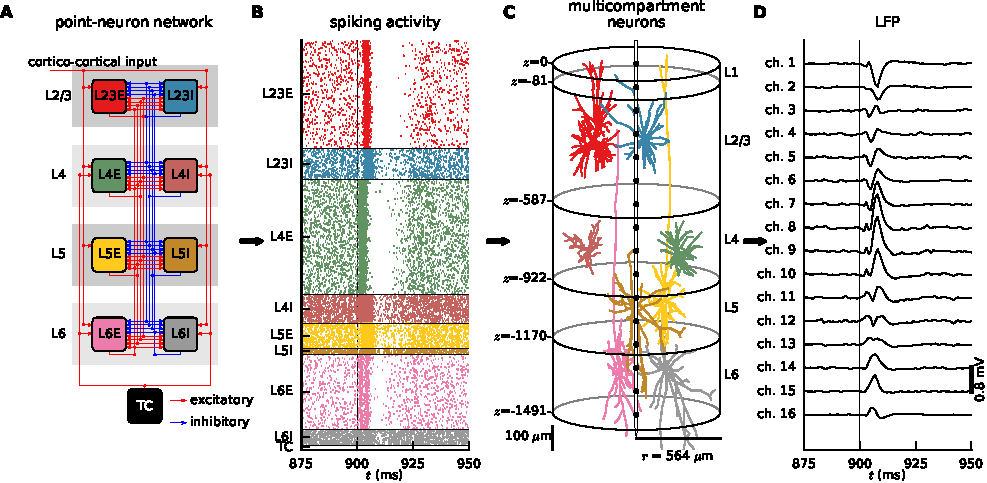
\includegraphics[width=\columnwidth]{Figures/Ch-LFPy/hybridmodel}
\caption{\ehnote{Hagen 2016 caption:}
Overview of the hybrid LFP modeling scheme for a cortical microcircuit model.
(A) Sketch of the point-neuron network representing a
\SI{1}{\milli\metre} patch of early sensory cortex (adapted from Potjans2014).
The network consists of 8 populations of LIF neurons, representing excitatory (E) and inhibitory neurons (I) in cortical layers 2/3, 4, 5, and 6.
External input is provided by a population of TC neurons and cortico-cortical afferents.
The color coding of neuron populations is used consistently throughout this paper.
Red arrows: excitatory connections. Blue arrows: inhibitory connections.
See Tables 1-2, 5-6 for details on the network model.
(B) Spontaneous (t < \SI{900}{\milli\second}) and stimulus-evoked spiking activity (synchronous firing of TC neurons at time $t = $\SI{900}{\milli\second}, denoted by thin vertical line) generated by the point-neuron network model shown in panel A, sampled from all neurons in each population. Each dot represents the spike time of a particular neuron.
(C) Populations of LFP-generating multicompartment model neurons with reconstructed, layer- and cell-type specific morphologies.
Cells are distributed within a cylinder spanning the cortex. Layer boundaries are marked by horizontal black lines (at depths $z$ relative to cortex surface $z = 0$). Only one representative neuron for each population is shown
(see Fig. 4 for a detailed overview of cell types and morphologies).
Sketch of a laminar recording electrode (gray) with 16 contacts separated by \SI{100}{\micro\metre} (black dots).
(D) Depth-resolved LFP traces predicted by the model (cf. Tables 3 and 4).
Note that channel 1 is at the pial surface, so that channel 2 corresponds to a cortical depth of \SI{100}{\micro\metre} and so forth.
}
\label{fig:LFPy:hybridmodel}
\end{center}
\end{figure}



One main assumption is that point-neuron network models can accurately capture observations present in experimental data gathered \textit{in vivo},
including irregular firing patterns
\ehnote{(Softky and Koch 1993; van Vreeswijk and Sompolinsky 1996; Amit and Brunel 1997; Shadlen and Newsome 1998), membrane-potential fluctuations (Destexhe and Pare 1999), asynchronous firing (Ecker et al. 2010; Renart et al. 2010; Ostojic 2014), correlations in neural activity (Gentet et al. 2010; Okun and Lampl 2008; Helias et al. 2013), self-sustained activity (Ohbayashi et al. 2003; Kriener et al. 2014), and realistic firing rates across laminar cortical populations (Potjans and Diesmann 2014).}
Similarly, reduced models derived from biophysically detailed multicompartment neuron models has shown that point-neuron network models can accurately capture spiking statistics of the biophysically detailed model variants (see e.g., \cite**{Roessert2016,Billeh_2020}).
In the case of \cite**{Roessert2016} the effect of dendritic filtering on synaptic input currents is captured by computing an equivalent filter for each possible synapse location and type using a Green's function formalism \cite**{Wybo_2013}.
The point neurons are modeled using a generalized integrate-and-fire (GIF) formalism,
and the linear filters applied to the synaptic currents result in  well-preserved post-synaptic potentials in the point neuron. \ehnote{perhaps I'll leave this last point out.}

Another main assumption underlying the hybrid scheme is that spatial information, that is, neuronal geometry and locations of synapses can be incorporated for the purpose of computing extracellular signals,
based on rules derived from available anatomical knowledge.
This assumption entails that a point-neuron network population representing for instance a set of layer 5 pyramidal cells,
will be represented by a corresponding population of geometrically detailed multicompartment neuron models,
placed at a cortical depth and density in accordance with the overall network size and available anatomical constraints.
Similarly, incoming synaptic connections onto the same point-neuron population from each presynaptic population,
for instance layer 4 inhibitory interneurons,
should be positioned onto the layer 5 pyramidal cell geometries according to rules derived from available data on such connections,
while also preserving the typical number of incoming synapses (aka synaptic in-degree).

In the original application of the hybrid scheme \cite**{Hagen2016} to a point-neuron network model representing a generic cortical microcircuit \cite**{Potjans2014},
a number of parameters of the network model were inherited by the  forward-modeling step.
In order to preserve synaptic currents,
the same current-based synapse type (see \Fref{sec:Ch-Neuron:current-based-syn}) with an exponentially decaying temporal kernel were used,
with the same average maximum current amplitude,
and with activation delays drawn from the same conduction delay distribution as was used in the network.
Synapse sites on the postsynaptic morphologies were derived from a connectivity dataset resolving numbers of synapses per layer between 16 different excitatory and inhibitory neuron types spanning layers 2/3, 4, 5 and 6.
The total numbers of synapses per connection (from each presynaptic to postsynaptic population) were preserved.
Furthermore, membrane time constants of the reconstructed morphologies which utilized purely passive compartments throughout were set similar to those of the point neurons.
\ehnote{kunne lagt til noe om ekspandering av enkelte punktnevronpopulasjoner til forskjellige celletyper som vi gjorde den gang.}


\subsubsection{Hybrid scheme -- step by step}
\ghnote{Tanke: Er det mulig aa heller skrive dette som en kokebokoppskrift - punktlister for Step 1, Step 2, og Step 3 (som vel er bankers) foerst, og saa ta all diskusjon om eventuell validitet til slutt? Slik det staar blir det saapass mange forbehold introdusert underveis at det er lett aa miste traaden. Den foerste store lista (under) er ei liste over noe som egentlig ikke brukes direkte i hybrid-skjemaet. Den brukes kun under en validering som gaar ut paa aa bytte ut Step 1 med en ordentlig MC-simulering? Jeg tenker at kokebokoppskriften boer komme i forgrunnen. }

One key feature of the this hybrid scheme application as devised by \cite**{Hagen2016} was an assumed-to-be \emph{linear} spike-LFP relationship, that is, one spike generated by a network subpopulation would result in a fixed contribution to the extracellular signal resulting from synaptic and transmembrane currents on postsynaptic multicompartment neurons.
So how can we make an argument about the validity of said scheme,
e.g., in the presence of \emph{non-linear} synaptic and ion-specific channels?
Conceptually, it is perhaps best to \emph{first} consider a recurrently connected network of biophysically detailed neurons which allows for computing extracellular signals,
and that the aforementioned point-neuron network model represents something of an idealized scenario obtained by reducing biophysical detail in a systematic manner.

Let us first define some properties of the biophysically detailed model, as general as possible. 
For compactness, 

\begin{enumerate}
\item Let $X \in \{ \ldots \}$ and $Y \subseteq X$ denote pre- and postsynaptic population, respectively. Each population corresponds to separate classes of neurons (derived from anatomy, electrical properties, gene expression etc.).
\item Let $N_X$ and $N_Y$ denote the sizes of population $X$ and $Y$.
\item Let $u \in \{ 1, \ldots , N_X \}$ and $v \in \{ 1, \ldots , N_Y \}$ denote pre- and postsynaptic neuron index, respectively.
\item Let $\mathbf{r}_u \sim \widetilde{\mathbf{r}}_X$ denote the discretely sampled somatic location of neuron $u$,
where $\widetilde{\mathbf{r}}_X$ describes the probability density function of somatic locations of population $X$ in space.
\item Let $K_{YX}$ denote the total number of synapses between presynaptic population $X$ and postsynaptic population $Y$.
Assuming a random connectivity with binomial in- and out-degree distributions the corresponding connection probability is then $C_{YX}=1-(1-1/{N_Y N_X})^{K_{YX}}$ \cite**{Potjans2014}.
For small connection probabilities the expression can be approximated by $C_{YX} = K_{YX} / (N_Y N_X)$.
\item Let layer or region (e.g., cortical layer) be denoted by $L$.
\item Let synapse placement be described by a spatial probability function $\mathcal{L}_{YXL} \geq 0 $ such that $\sum_L \mathcal{L}_{YXL} \coloneq 1$ if $K_{YX} > 0$ and 0 if $K_{YX} = 0$.
Connection probabilities may also depend on both spatial location and/or properties of the postsynaptic neurons such as compartment surface areas $\mathbf{A}_Y$.
\item Synaptic currents for each connection are given as $I_{\mathrm{syn}YX}(t)=\overline{G}_{\mathrm{syn}YX} f_{YX}(t)(V_\mathrm{m}(t)-E_{\mathrm{syn}X})$
where $\overline{G}_{\mathrm{syn}YX}$ denotes the maximum synaptic conductance and $f_{YX}(t) \in [0, 1]$ one of the temporal kernels listed in \Fref{sec:Ch-Neuron:conductance-based-synapses}.
$V_\mathrm{m}(t)$ denotes the postsynaptic potential and $E_{\mathrm{syn}X}$ denotes the reversal potential of the synapse which is determined by the presynaptic cell type (i.e., excitatory or inhibitory).
For simplicity we will assume that $\overline{G}_{\mathrm{syn}YX}$ is independent of $L$.
We will also assume that connection weights $\overline{G}_{\mathrm{syn}YX}$ are static, 
that is, there are no synaptic plasticity rules in place.
\item Let the conduction delays resulting from presynaptic action potential generation time  to activation time of the synapse be greater than zero and randomly drawn from some function as $\Delta_{vu} \sim \widetilde{\Delta}_{YX}(t)$.
For simplicity, we let conduction delays be independent of cell location and geometry.
(Other use cases may also compute delays based on distance between pre- and post-synaptic units assuming a typical value for axonal action potential propagation speed.)
\item Each postsynaptic neuron $v \in Y$ is modeled using the  `standard' multicompartment neuron formalism such that their transmembrane currents $\mathbf{I}_\mathrm{m}^{\langle v \rangle}(t)$ or axial currents $\mathbb{I}_\mathrm{a}^{\langle v \rangle}(t)$ can be computed.
Here $X$ and $Y$ may be used interchangeably, however,
presynaptic populations may also include, remote populations, point processes, external stimuli and similar,
which we will assume give approximately zero direct contributions to the signals predicted by the full recurrent network model.
\item Extracellular signal contributions in different spatial locations may be computed and summed up as
$\sum_Y \sum_{v=1}^{N_Y} \mathbf{F}^{\langle v \rangle} \mathbf{I}_\mathrm{m}^{\langle v \rangle}$ and similar for axial currents.
$\mathbf{F}^{\langle v \rangle}$ here denotes a linear mapping of transmembrane currents of cell $v$ to a linearly dependent signal.
\item The sequence of spike times $s_u(t) = \sum_k \delta (t - t_k)$ of each of each neuron $u \in X$ is recorded throughout the entire simulation interval $[0, t_\mathrm{sim} \rangle$.
We may choose to relax this requirement if a population $X$ represents an external population feeding persistent, uncorrelated events with spectrally `flat' spiking statistics (e.g., fixed-rate Poisson point processes) into the recurrently connected network.
\item We may store the weighted, directed graph representing vertices (connections) between nodes (neurons) for every pair of pre- and postsynaptic populations.
This requirement may also be relaxed if the total number of connections $K = \sum_X \sum_Y K_{YX}$ is large enough to make storage infeasible or one could recreate the full connectivity graph procedurally (at least statistically).
Graph weights represent maximum synaptic conductances.
The graph must also include the synaptic locations on the postsynaptic neurons. 
We will hereby let compartment index $w$ equate synaptic location.
\end{enumerate}


\begin{figure}[!ht]
\begin{center}
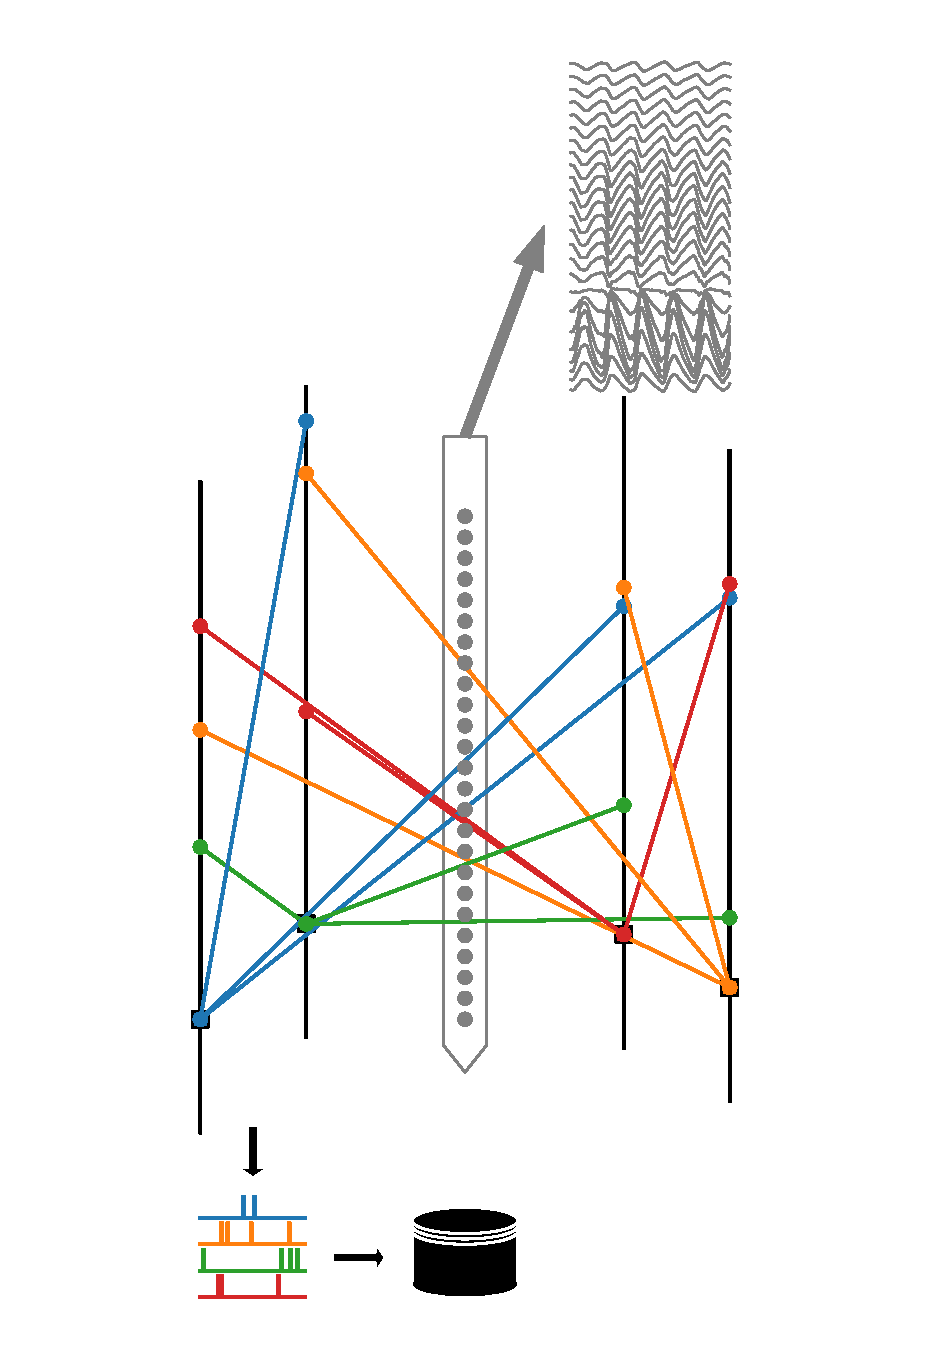
\includegraphics[width=0.49\textwidth]{Figures/Ch-LFPy/Ch-LFPy-hybrid_A.pdf}
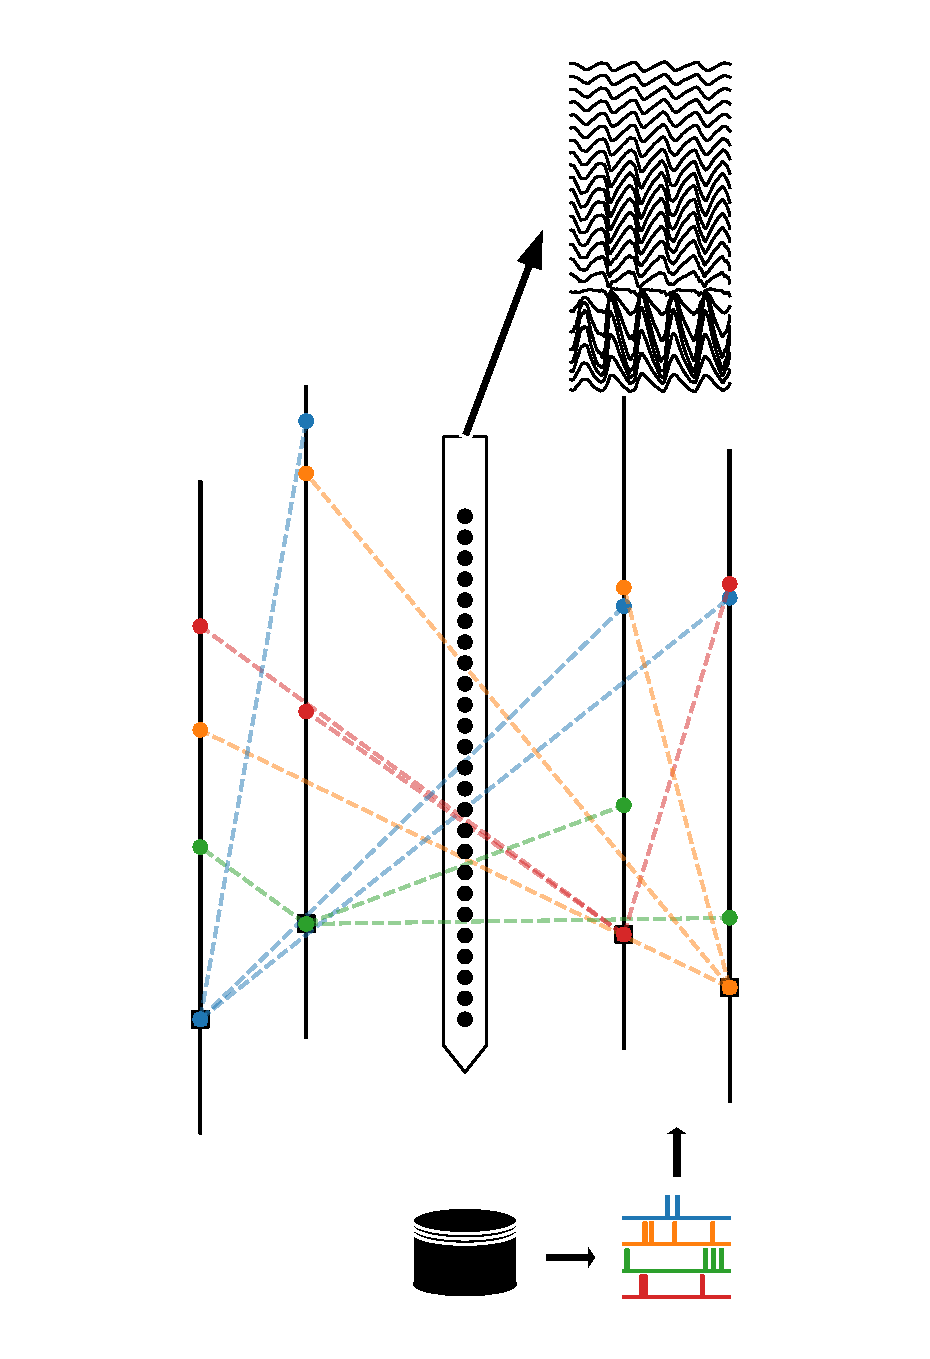
\includegraphics[width=0.49\textwidth]{Figures/Ch-LFPy/Ch-LFPy-hybrid_B.pdf}
\end{center}
\caption{\textbf{Disassociation between simulations of network activity and extracellular potentials.}
({\bf A}) Illustration of self-consistent multicompartment neuron network simulation where the primary output are single-unit spike trains (bottom left),
which is in turn stored in a database or file (bottom).
Extracellular potentials can optionally be computed,
here illustrated by the laminar probe outlined in gray.
Outgoing colored lines from each ball-and-stick neuron model denotes a connection from the soma of presynaptic neurons to synapses distributed on postsynaptic neurons.
({\bf B}) `Hybrid` simulation where recurrent network connections (dashed lines) have been removed,
but synaptic locations have been preserved.
Here, synaptic activation times are set from pre-recorded spike times recorded to a database (bottom).
The synaptic currents and associated transmembrane currents on the postsynaptic neurons allows for computing the extracellular potential independently of the recurrent network dynamics.
}
\label{fig:LFPy_hybrid}
\end{figure}


\begin{figure}[!ht]
\begin{center}
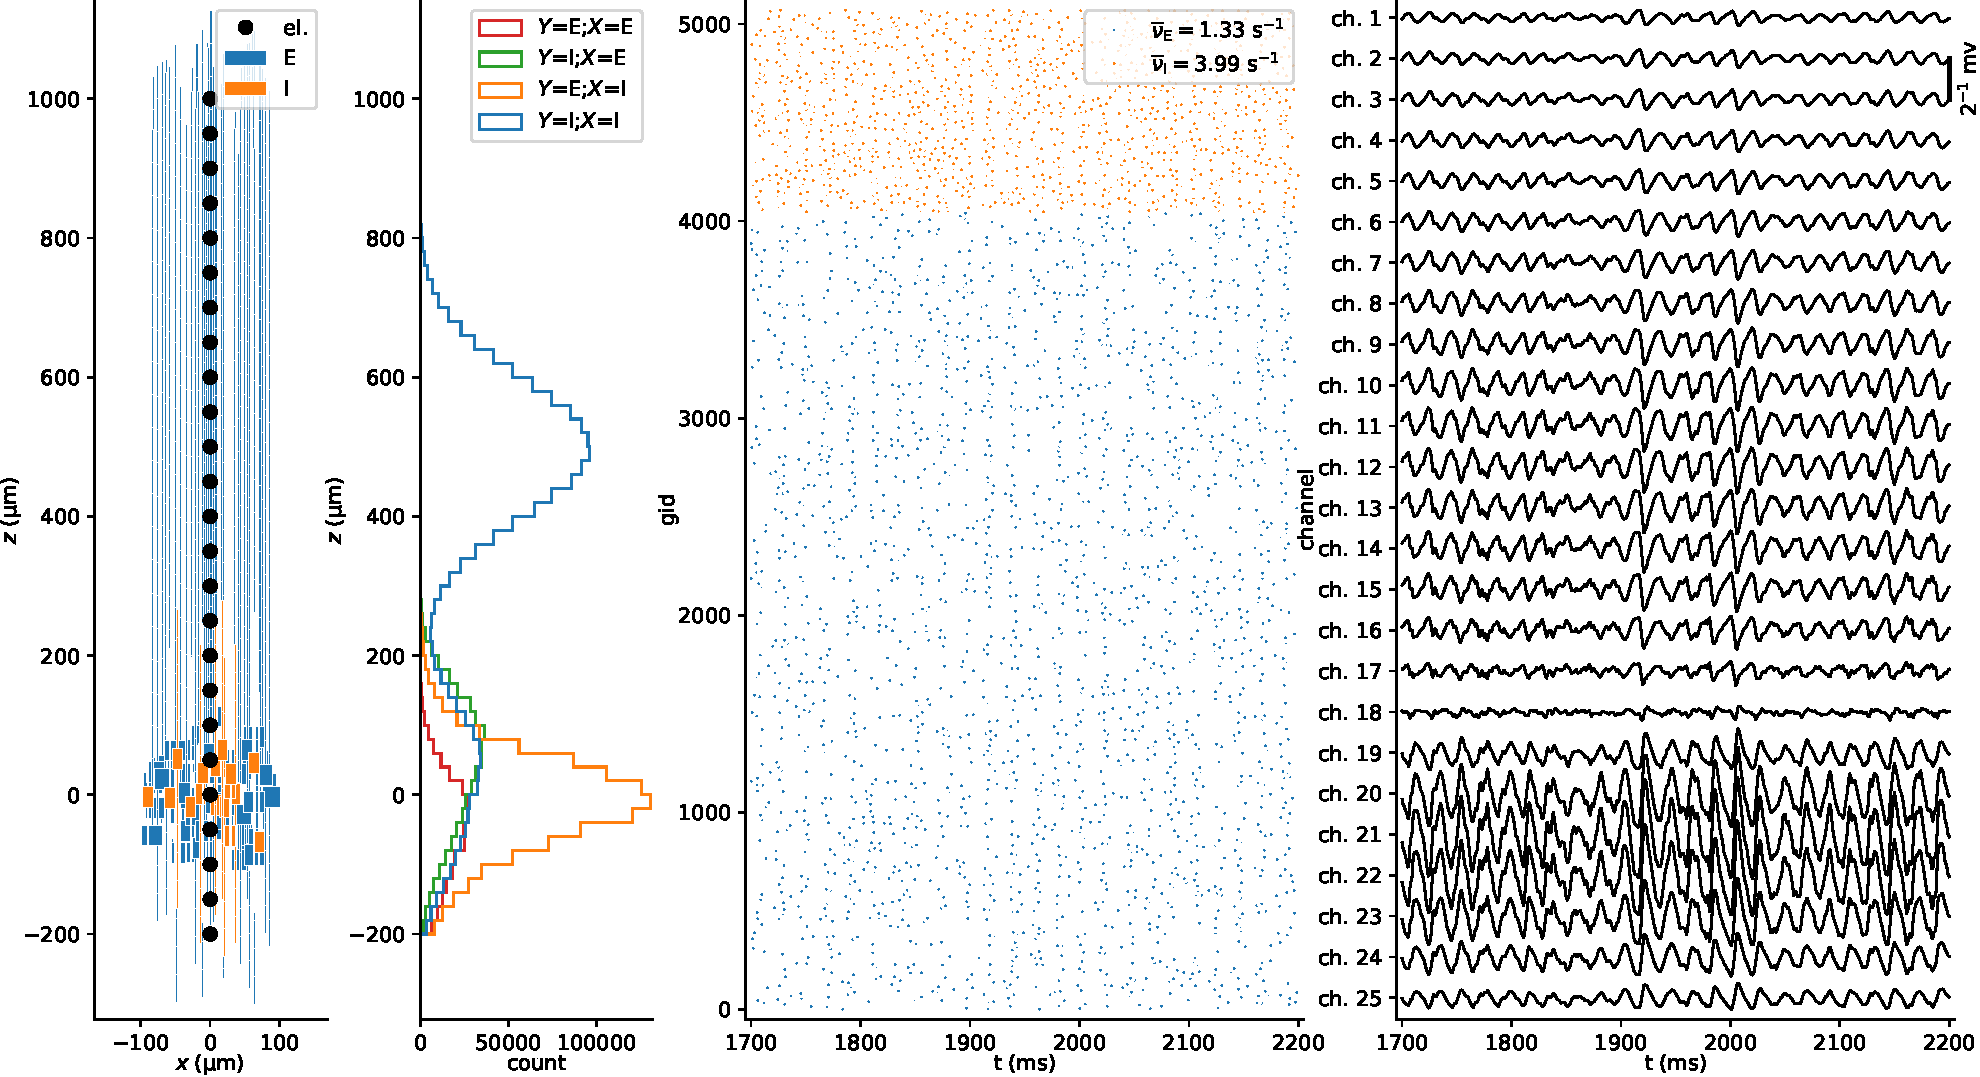
\includegraphics[width=\textwidth]{Figures/Ch-LFPy/Ch-LFPy-network.pdf}
\end{center}
\caption{\textbf{Stylized two-population multicompartment neuron network with predictions of extracellular potentials.}
({\bf A}) Cell and electrode geometry. The network is constructed of one excitatory (`E') and one inhibitory (`I') population.
Only a subset of cells are shown from each population.
The black point markers along the $z$-axis denote locations of electrode contact points with separation \SI{50}{\micro\metre}. 
({\bf B}) Synapse counts per connection $K_{YX}$ along the vertical $z$-axis in bins of \SI{20}{\micro\metre}.
({\bf C}) Network spike raster spanning \SI{500}{\milli\second} of spontaneous activity. 
The mean population-averaged firing rates are given shown in the legend.
({\bf D}) Per-population spike-count histograms with bin size \SI{5}{\milli\second}.
({\bf E}) Extracellular potentials.
\ehnote{legg til panel labels}
}
\label{fig:LFPy_network}
\end{figure}




At this point one could destroy every connection of the recurrently connected network,
load sets of spike events $s_u(t)$ of presynaptic neurons $u \in X$ recorded to some intermediate data storage,
reinstate every synapse on each postsynaptic neuron $v \in Y$ but this time activate them at times
$\left(s_u(t) \ast \delta(t-\Delta_{vu})\right)$
accounting for transmission delay,
and otherwise keep neuron and synapse parameterization and locations the same.
The asterisk symbol denotes a convolution operation.
This would result in exactly the same changes in membrane voltages and consequently the same spatiotemporal distributions of transmembrane currents as in the recurrently connected case.
However, what did we gain through these steps?

\begin{enumerate}
\item Full disassociation of simulations of neuronal network dynamics and simulations of extracellular signals,
as illustrated in \Fref{fig:LFPy_hybrid}.
\item HPC resources may have been required for simulating neural dynamics in the recurrently connected network in parallel in the first place,
but one may now utilize a trivial parallelization scheme in order to compute extracellular signals as contributions of each cell is independent of the others.
One could even do each single-cell simulation serially.
\item Little was gained in terms of overall computational cost -- the total number of state variables (for active ion channels etc.) remains approximately the same.
The computational cost of transmitting times of spike events across a recurrent network can be assumed to be minuscular compared to solving for the membrane potentials and extracellular potentials, etc.
\end{enumerate}

For the purpose of predicting extracellular signals \emph{only}, let us now do some model simplification -- assuming we can preserve the spatiotemporal distributions of transmembrane currents on average. We will also relax the requirement \ghnote{Har dette blitt satt opp som et requirement som kan relaxes? We will not require that ....?} that postsynaptic neurons in the hybrid scheme predict correct action potential times (or in fact \emph{any} action potentials or correct membrane potential statistics at all): \ghnote{Kan det beskrives tydeligere hva vi her faar en liste over. Det som foelger er MC modellen vi skal mate spike-times inn i.}

\begin{enumerate}
\item Approximate conductance-based synapses by equivalent current-based synapses:
\begin{eqnarray}
I_{\mathrm{syn}YX}(t)
	&=& \overline{G}_{\mathrm{syn}YX}f_{YX}(t)\left(V_\mathrm{m}(t) - E_{\mathrm{syn}X}\right) \\
	&\approx& \overline{G}_{\mathrm{syn}YX}f_{YX}(t)\left(\langle V_\mathrm{m}(t) \rangle - E_{\mathrm{syn}X}\right) \\
	&=& \overline{I}_{\mathrm{syn}YX}f_{YX}(t)~,
\end{eqnarray}
where $\langle V_\mathrm{m}(t) \rangle$ denotes the spatiotemporally averaged postsynaptic potential (or its expectation value).
We here use the sub-fix $YX$ notation to emphasize that some of these parameters may be connection specific.
We would also note that some rescaling of current amplitudes \emph{may} be required for certain synapse instances if the postsynaptic targets are characterized by very high input impedances (e.g., oblique dendrites).

\item In absence of conductance-based synapses, incorporate the \emph{effective membrane conductance} $G_\mathrm{eff}$.
\ghnote{Incorporate faar det til aa virke som om denne settes inn blant andre. Er det bedre med noe ala: "replace all present membrane conductances in terms of a single effective membrane conductance?"} \ghtxt{\sout{Ignoring other conductances which may be present (active ion channels etc.) except the passive leak conductance, } Assuming it depends only on synaptic currents and the passive leakage current,} the total membrane conductance per postsynaptic compartment $w$ is
\begin{equation}
G_{\mathrm{tot}}(t) = G_L + \sum_X \sum_{u \subset X} \overline{G}_{\mathrm{syn}YX} \left( f_{YX} \ast s_u \ast \delta(t-\Delta_{vu}) \right)(t)
\end{equation}
where $G_L \coloneq g_L A_w$ is the total leak conductance from the specific conductivity $g_L$ and compartment area $A_w$, $s_u(t)$ the sequence of presynaptic spikes and $\Delta_{vu}$ the conduction delay. The double sum over presynaptic populations $X$ and units $u \in X$ \ghtxt{\sout{imply}implies} that each presynaptic unit targeting the compartment is accounted for. Assuming a fixed average presynaptic spike rate $\langle \nu_u \rangle \coloneq \Delta t^{-1} \int_t^{t+\Delta t} s_u(t) dt$ for any time duration $\Delta t$ and a normalized delay distribution ($\int_0^\infty \widetilde{\Delta}_{YX}(t) dt \coloneq 1$), the time-averaged effective conductance is approximately
\begin{equation}
G_\mathrm{eff} \coloneq \langle G_\mathrm{tot}(t) \rangle \approx G_L + \sum_X \sum_{u \subset X} \langle \nu_u \rangle \overline{G}_{\mathrm{syn}YX} \int_0^\infty f_{YX}(t) dt ~.
\end{equation}

\item Remove active ion channels if their net contributions to the total transmembrane currents can be assumed to be small around typical membrane voltage values. \ghnote{Kan ikke dette angis som en parantes i punktet nedenfor. Disse kan vel lineariseres som alle andre?}

\item Active ion channel currents on the specific form
\begin{equation}
i_\mathrm{w}(t) = - \overline{g}_\mathrm{w} \omega(t)\left( V_\mathrm{m}(t) - E_\mathrm{w} \right)~ \label{eq:Ch-LFPy:active}
\end{equation}
may be \ghnote{May be or are?} approximated by equivalent, linearly dependent currents \cite**{Remme_2010,Ness2016} if their maximum \ghtxt{\sout{conductivity}conductance} $\overline{g}_\mathrm{w}$ is significant. \ghnote{Jmf. punkt over - her kan man kanskje si if g is significant, or ignored if not?} Here, $E_\mathrm{w}$ is the channel reversal potential and
$\omega(t)$ the gating variable which dynamics are given in terms of an activation time function $\tau_\mathrm{w}(V)$ and activation function $\omega_\infty(V)$ as
\begin{equation}
\tau_\mathrm{w}(V_\mathrm{m}(t)) \frac{\partial\omega(t)}{\partial t} = \omega_\infty(V_\mathrm{m}(t)) - \omega(t)~.
\label{eq:Ch-LFPy:domega_dt}
\end{equation}
If the voltage dynamics of the active compartment is defined by
\begin{equation}
c_\mathrm{m}\frac{\partial V_\mathrm{m}(t)}{\partial t} =
	- \overline{g}_\mathrm{L}\left(V_\mathrm{m}(t) - E_\mathrm{L}\right)
	- \overline{g}_\mathrm{w}\omega(t)\left(V_\mathrm{m}(t) - E_\mathrm{w}\right)
	+ I_\mathrm{a}~,
\end{equation}
one can obtain the so-called \emph{quasi-active approximation} \cite**{Koch1984,Remme_2010,Ness2016} by linearizing each voltage dependent term around the steady state value $\langle V_\mathrm{m}(t) \rangle$ resulting in
\begin{eqnarray}
c_\mathrm{m}\frac{\partial V_\mathrm{m}(t)}{\partial t} &=&
	- g_\mathrm{L} \left( \gamma_\mathrm{R}
						  \left( V_\mathrm{m}(t) - \langle V_\mathrm{m}(t) \rangle \right)
						  + \eta m(t)  \right)
	+ I_\mathrm{a} ~\text{, where} \\
\gamma_\mathrm{R} &\coloneq& 1 + \overline{g}_\mathrm{w} \omega_\infty(\langle V_\mathrm{m}(t) \rangle) / g_\mathrm{L} ~\text{, and} \\
\eta &\coloneq& \frac{\overline{g}_\mathrm{w} ( \langle V_\mathrm{m}(t) \rangle - E_\mathrm{w} )}{g_\mathrm{L}} \frac{\partial\omega_\infty (\langle V_\mathrm{m}(t) \rangle)}{\partial V_\mathrm{m}}~.
\end{eqnarray}
\ghnote{Overline forsvinner fra konduktansene underveis.}
Here, an equivalent gating variable was defined as
\begin{equation}
m(t) \coloneq \left( \omega(t) - \omega_\infty ( \langle V_\mathrm{m}(t) \rangle ) \right) / \frac{\partial\omega_\infty (\langle V_\mathrm{m}(t) \rangle)}{\partial V_\mathrm{m}}~,
\end{equation}
and its linear dynamics is governed by
\begin{equation}
\tau_\mathrm{w} (\langle V_\mathrm{m}(t) \rangle) \frac{\partial m(t)}{\partial t} = V_\mathrm{m}(t) - \langle V_\mathrm{m}(t) \rangle - m(t)~.
\end{equation}
%
Above, $\gamma_\mathrm{R}$ denotes the ratio between the total and leak conductance
while $\eta$ characterize whether the quasi-active current approximation act as positive $(\eta < 0)$ or negative $(\eta > 0)$ feedback.
%
For the special case $\eta=0$ the quasi-active current is `frozen', acting as a static, passive current \cite**{Ness2016}.
\ehnote{@TBN; hva mente du egentlig naar du skrev dette? Den kvasi-aktive stroembidraget er vel lineaert avhengig av $V_\mathrm{m}(t)$ hvis $\eta=0$ og foelgelig ikke statisk.}
%
Note that the above sets of equations corresponds to channels usually modelled with a single state variable (e.g., Na$^+$- and h-type currents),
but generalize also to current types with more than one gating variable (e.g., Na$^+$- and K$^+$ type currents), see \cite**{Remme_2010} for details. \ghnote{Litt mye aa ha med teori for linearisering av ionekanaler som et enkelt punkt i denne punktlista. Er det noe vi skal ha et kapittel om i Neuron istedet? Eller noe som kan kortes ned, og las hvile paa referanser til andres arbeid?} 

\item The leak conductance $E_L$ is modified as
\begin{equation}
E_L^\text{mod} = \langle V_\mathrm{m}(t) \rangle + \sum_\mathrm{w} \frac{g_\mathrm{w} (\langle V_\mathrm{m}(t) \rangle - E_\mathrm{w})}{g_L} ~,
\end{equation}
which ensures that the resting potential of the quasi-active model is similar to that of the fully active model.
\ghnote{Henger ikke helt med. Hvor ble det av den effektive avg-konduktansen definert i punkt 2?}

\item Further reduction of number of state variables can be achieved by reducing the number of compartments per postsynaptic cell. This may indeed reduce the accuracy of membrane voltage predictions, but more so at higher frequencies due to the intrinsic dendritic filtering. Extracellular signals like the LFP, EEG and MEG however carry more power at lower frequencies and may be less affected. Reducing compartment counts also enforces replacing synaptic locations by their nearest suitable location.

\item Further reduction of number of state variables describing linearly summing synaptic currents can be achieved by having at most one synapse per connection type (from $X$ onto $Y$) per compartment.
It's activation times are defined as the concatenation of sequences $\left(s_u \ast \Delta_{vu} \right)(t)$ for the subset $u \subset X$ being presynaptic to neuron $v \subset Y$ at the original synapse site(s) located on  compartment $w$.

\item With the exception of spike measurements, most electric and magnetic signals of interest carry most power at comparably low frequencies ($\lesssim$\SI{1}{\kilo\hertz}).
Thus, the temporal step size ($\Delta t$) of the simulations can usually be multifold increased compared to $\Delta t$ in the actual network simulation without sacrificing much in terms of accuracy in the relevant low-frequency range.
The computational cost is inversely proportional to the temporal step size,
and a reasonable choice may be $\Delta t \lesssim \tau \in \{ \tau_\mathrm{m}, \tau_\mathrm{syn}, \tau_\mathrm{w}, \ldots \}$,
that is, shorter than the typical time constants for membranes, synapses, ion channels etc.

\end{enumerate}

\ehnote{Sammenlikning av prediksjoner med `hybrid scheme' vs. ground truth kommer sammen med kernel-prediksjoner} 



\begin{figure}[!ht]
\begin{center}
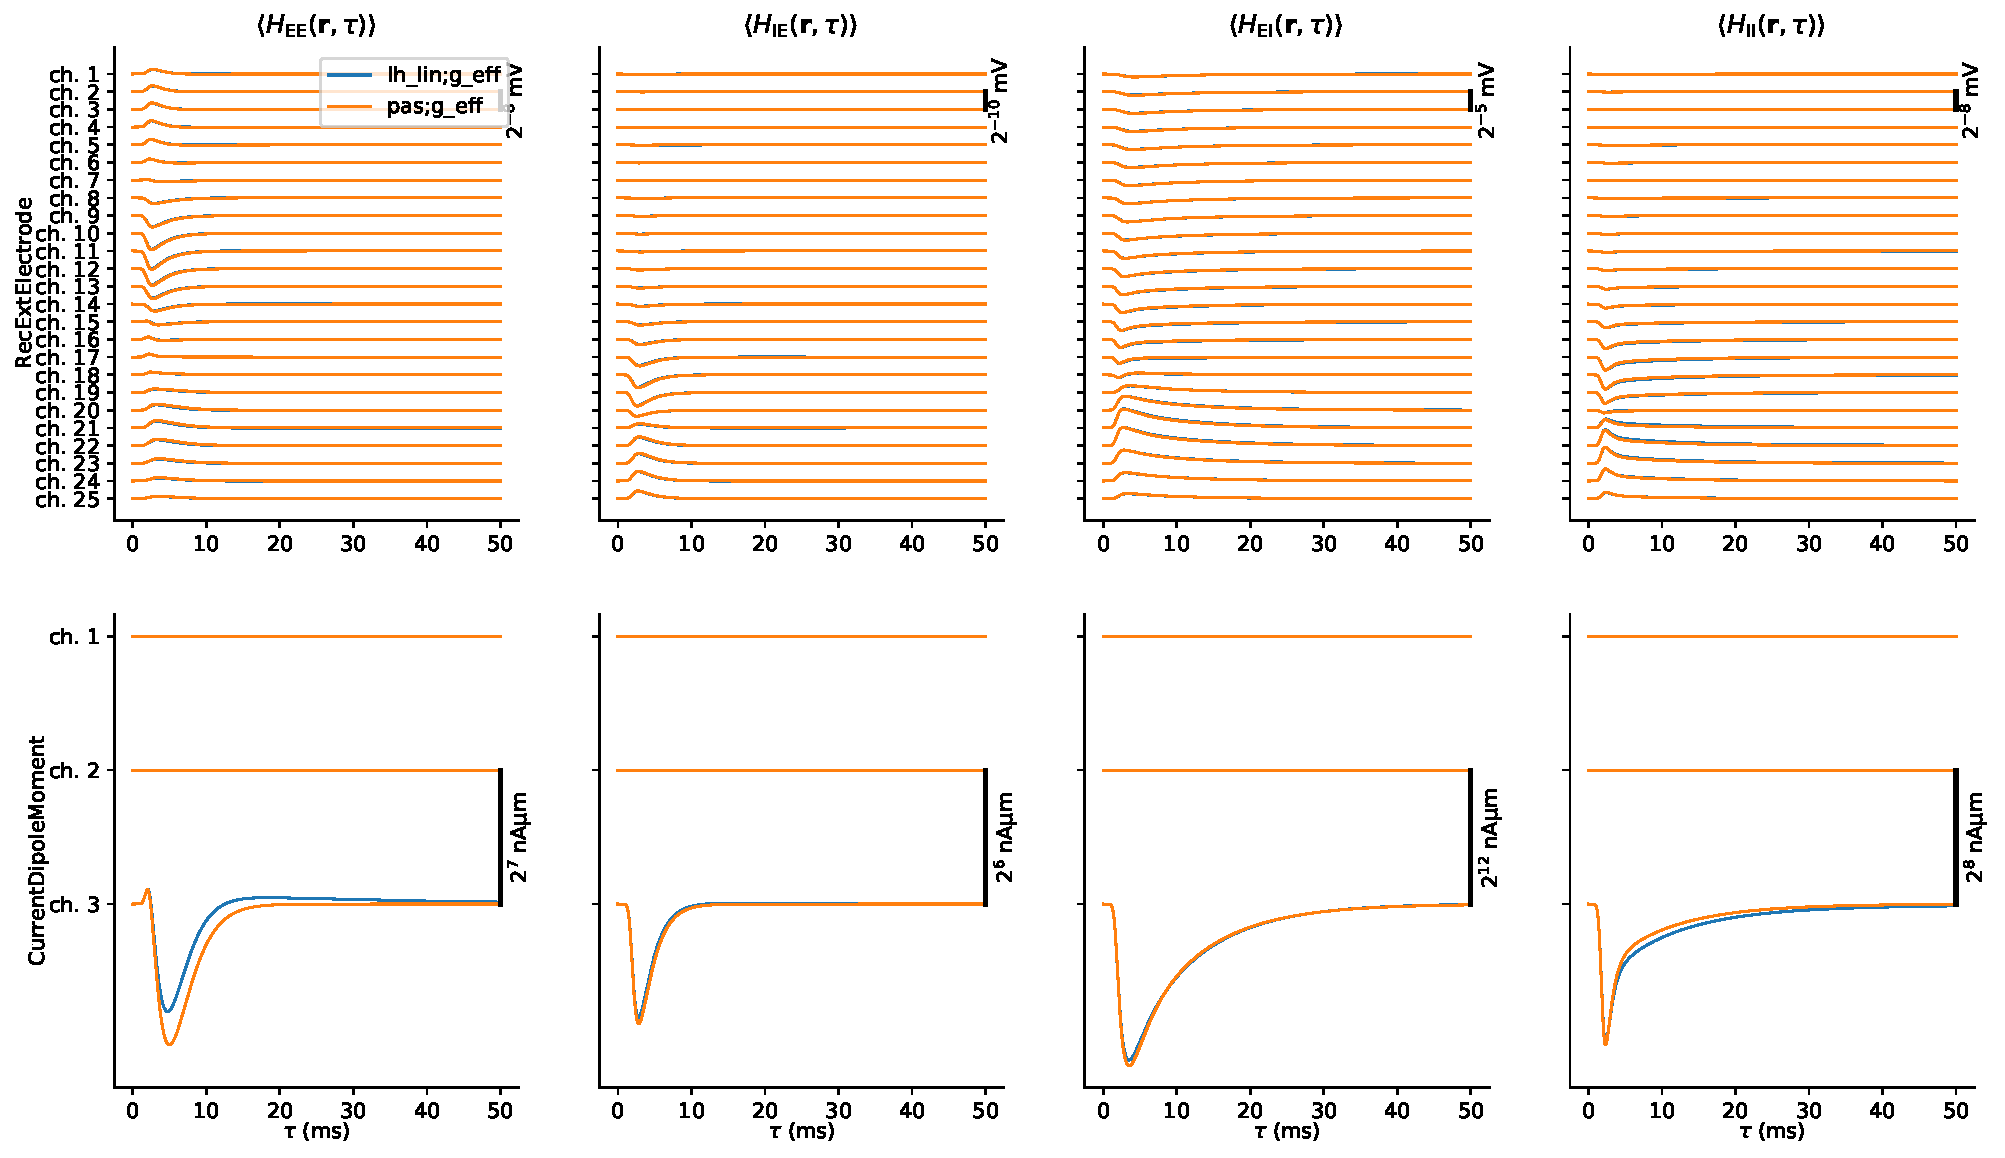
\includegraphics[width=\textwidth]{Figures/Ch-LFPy/Ch-LFPy-kernels.pdf}
\end{center}
\caption{\textbf{Spike-LFP impulse response functions (``kernels'').}
Spatiotemporal functions $\langle H_{YX}(\mathbf{r}, \tau) \rangle$ for each connection between every possible pre- and postsynaptic network population $X$ and $Y$, respectively.
The kernels are computed as the spike-averaged contribution by postsynaptic neurons to the extracellular potential in electrode contact locations shown in \Fref{fig:LFPy_network}{\bf A}.
The kernels are computed either using fully passive (`pas') or with quasi-linearized (`Ih\_lin') cable models.
\ehnote{placeholder - tenker fjerne current dipole moment.}
}
\label{fig:LFPy_kernels}
\end{figure}


\begin{figure}[!ht]
\begin{center}
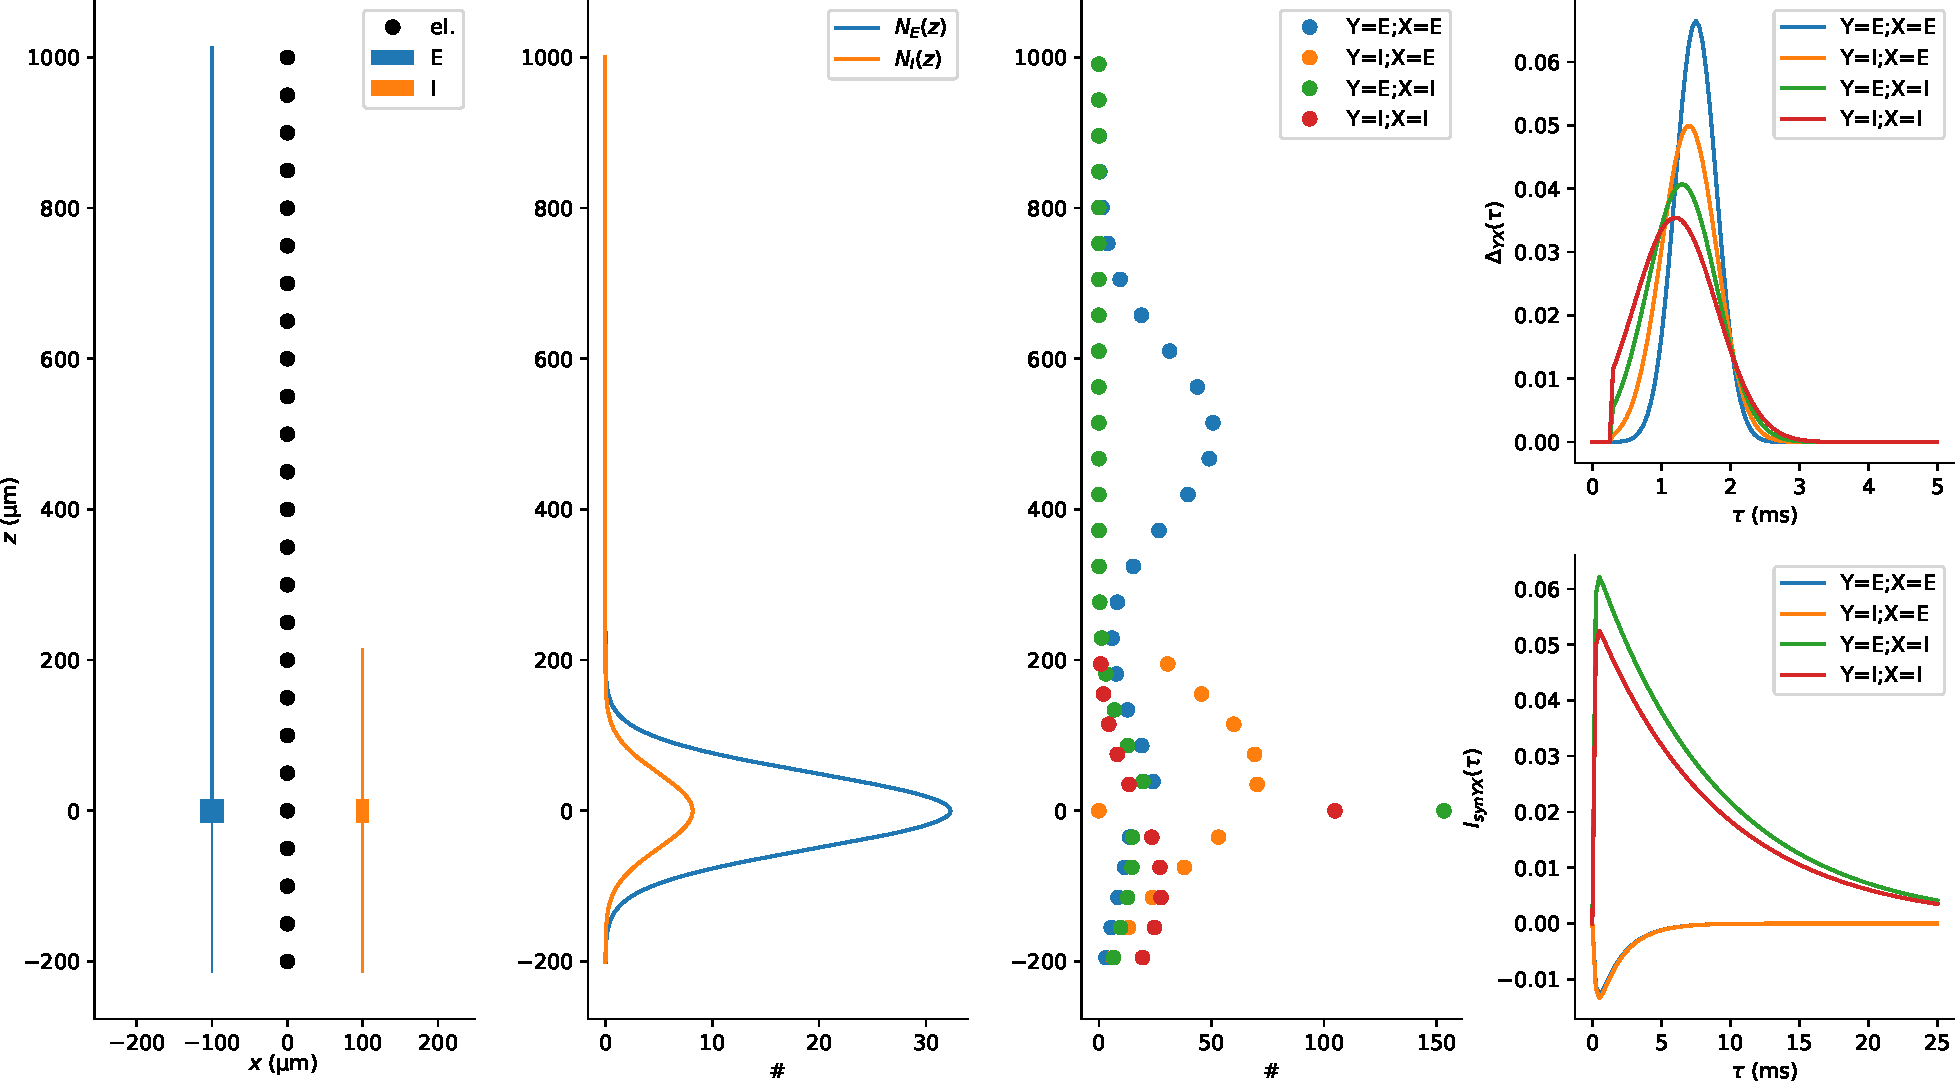
\includegraphics[width=\textwidth]{Figures/Ch-LFPy/Ch-LFPy-ratepredictor.pdf}
\end{center}
\caption{\textbf{Components for predictor of spike-signal filter kernels $\hat{H}_{YX}(\mathbf{r}, \tau)$.}
{\bf A} Multicompartment neuron models representative of each population `E' and `I',
with layout of extracellular laminar probe.
{\bf B} Densities of somas along $z$-axis.
{\bf C} Per-compartment synapse densities for each connection between the two populations.
{\bf D} Normalized distributions of transmission delays $\widetilde{\Delta}_{YX} (\tau)$ for each connection relative to presynaptic activation time.
{\bf E} Synaptic currents $I_{\mathrm{syn}YX}(\tau)$ relative to synaptic onset for each connection.
\ehnote{placeholder}
}
\label{fig:LFPy_kernel_predictor}
\end{figure}




\begin{figure}[!ht]
\begin{center}
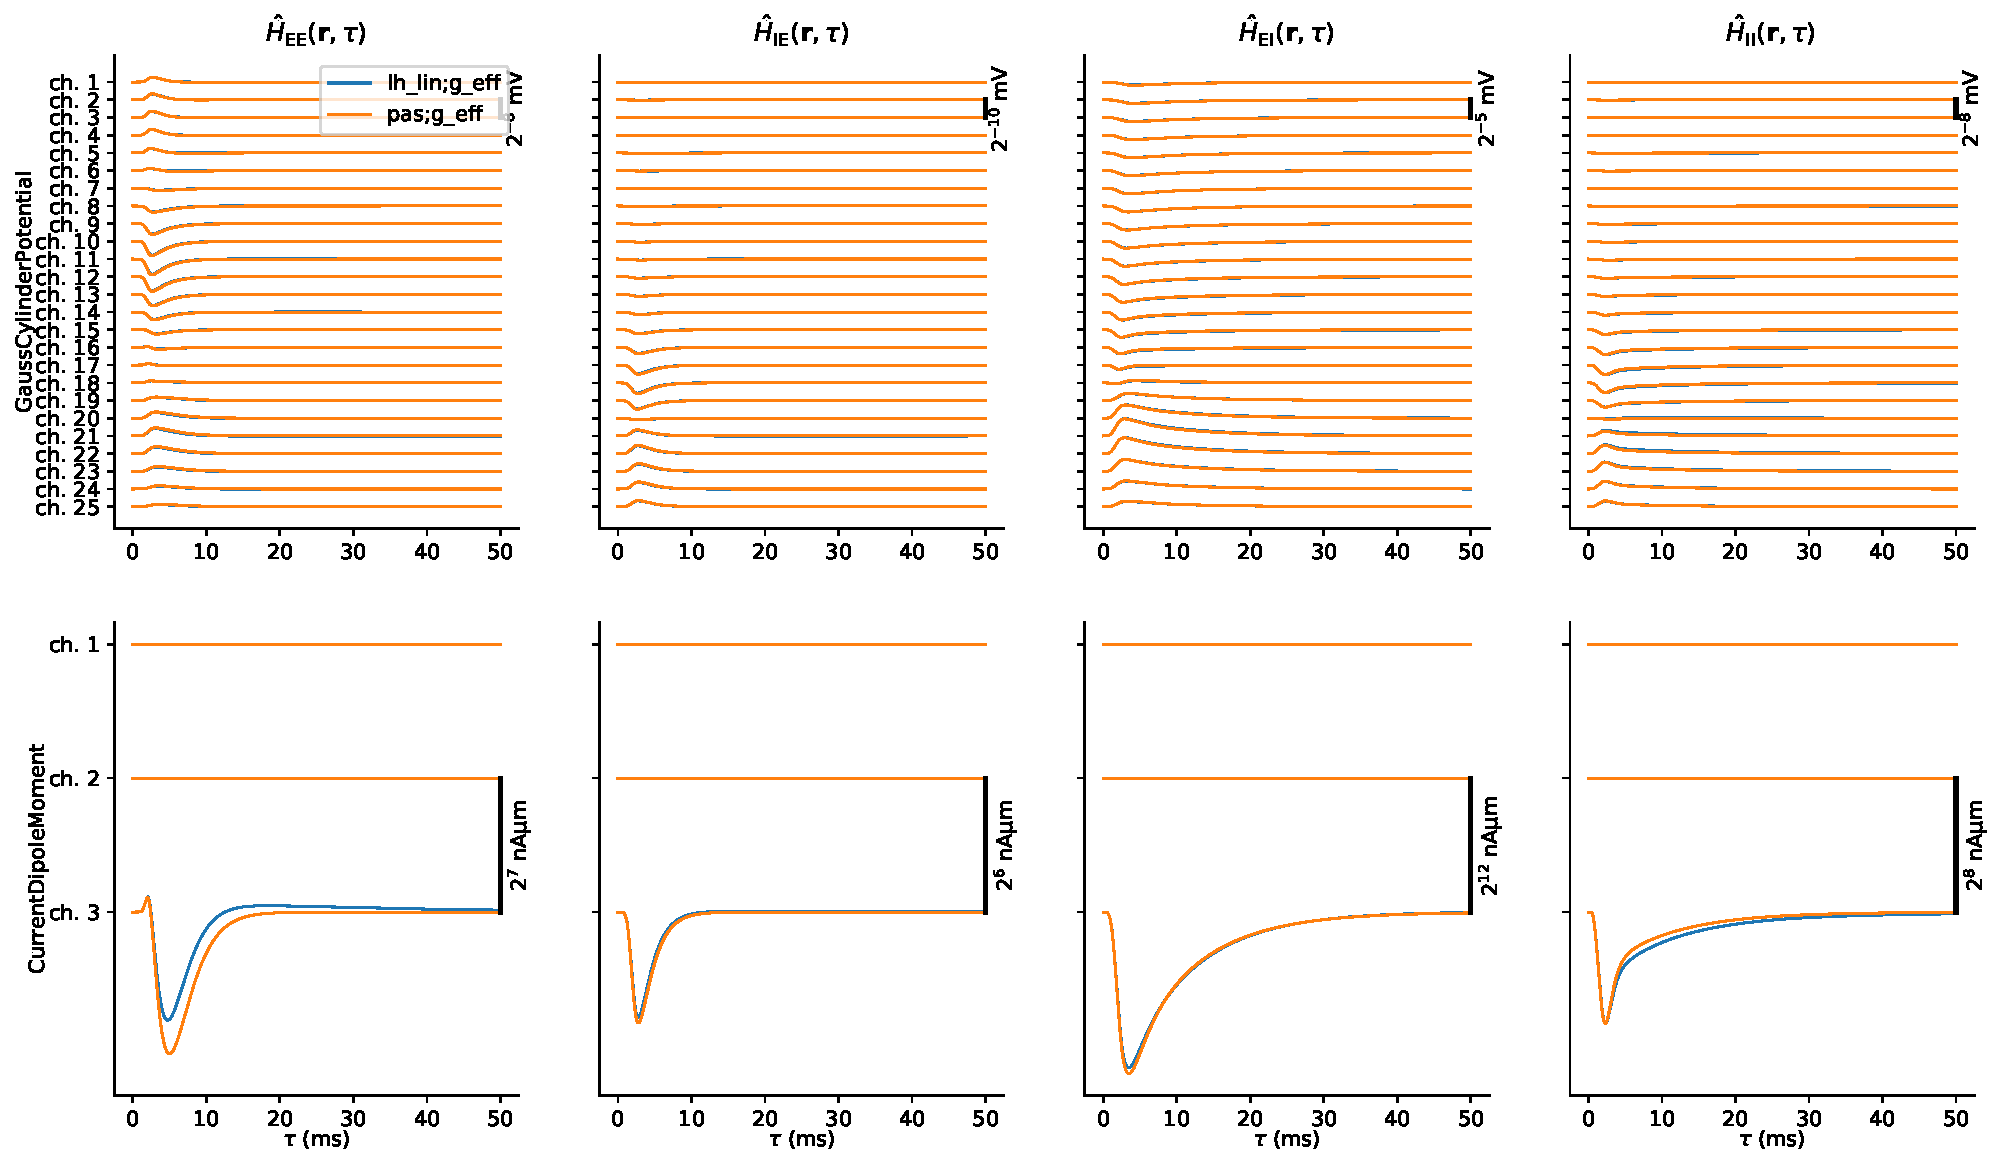
\includegraphics[width=\textwidth]{Figures/Ch-LFPy/Ch-LFPy-kernel_approx.pdf}
\end{center}
\caption{\textbf{Spike-LFP impulse response function predictions.}
Similar to \Fref{fig:LFPy_kernels},
but here computed using a computationally fast method accounting for the expectation values in terms of cell and synapse placement.
\ehnote{placeholder}
}
\label{fig:LFPy_kernel_predictions}
\end{figure}


\begin{figure}[!ht]
\begin{center}
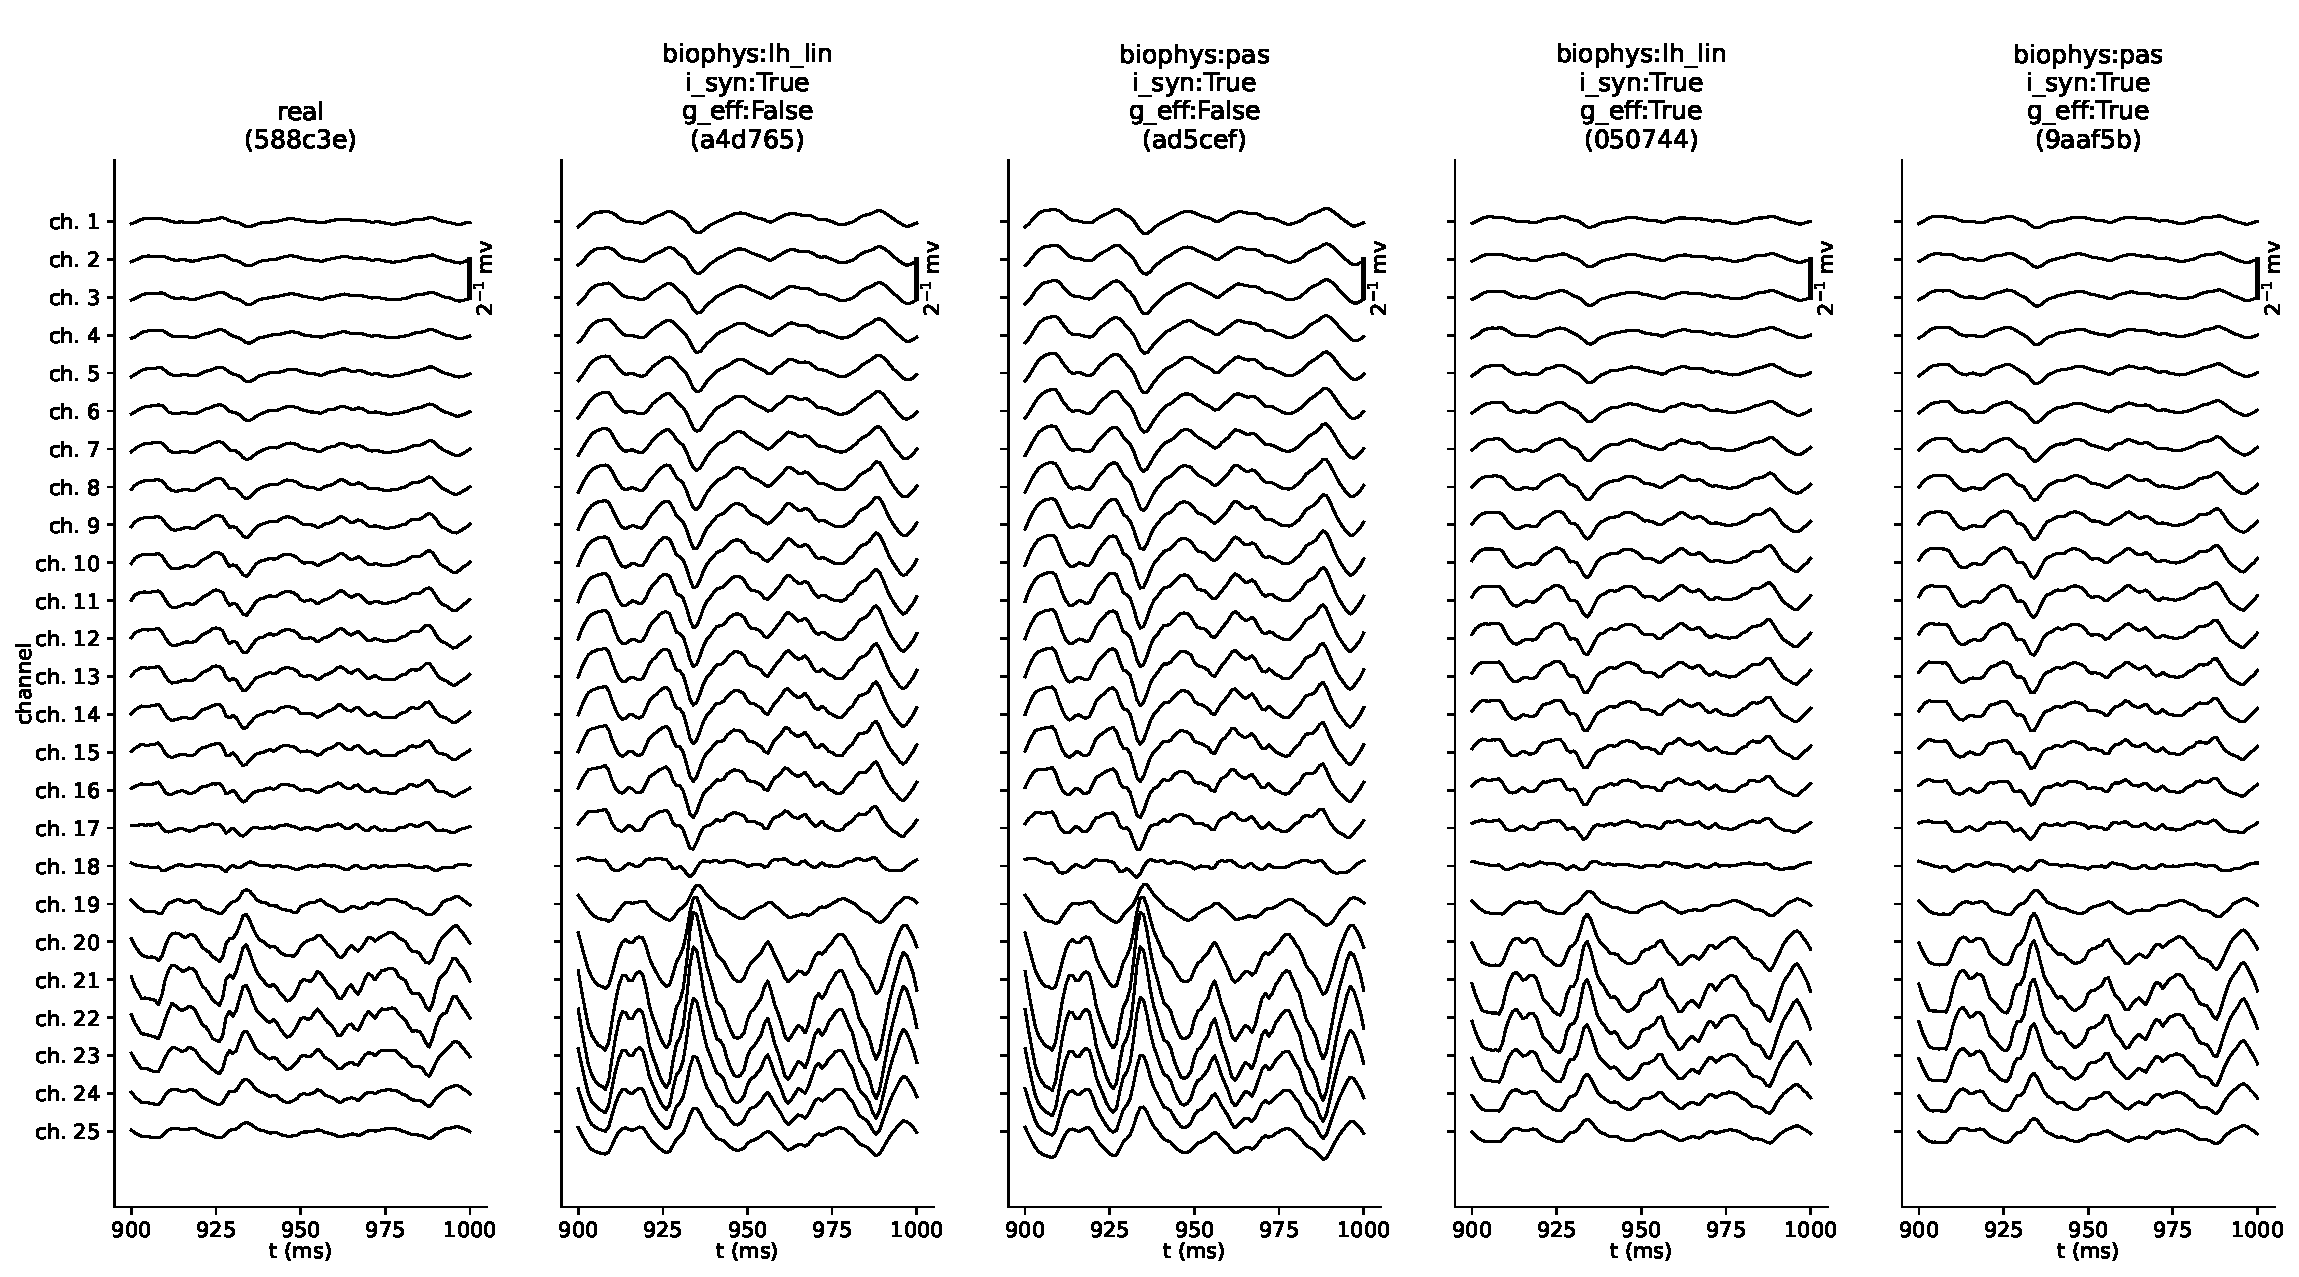
\includegraphics[width=\textwidth]{Figures/Ch-LFPy/Ch-LFPy-signal_vs_predictions.pdf}
\end{center}
\caption{\textbf{Ground truth signals vs. approximations.}
Here, extracellular potentials predicted from a multicompartment neuron network model (left) is compared to predictions made using the hybrid scheme (columns 2-5)
with either passive or quasi-linear multicompartment neurons,
ignoring or accounting for the effective membrane conductance (g\_eff=False/True respectively),
as well as kernel-based approximations obtained by convolving presynaptic population firing rates ($\nu_X(t)$) with respective kernels ($H_{YX}(\mathbf{r}, t)$) and summing the contributions (columns 6-9).
}
\label{fig:LFPy_predictions}
\end{figure}


\begin{figure}[!ht]
\begin{center}
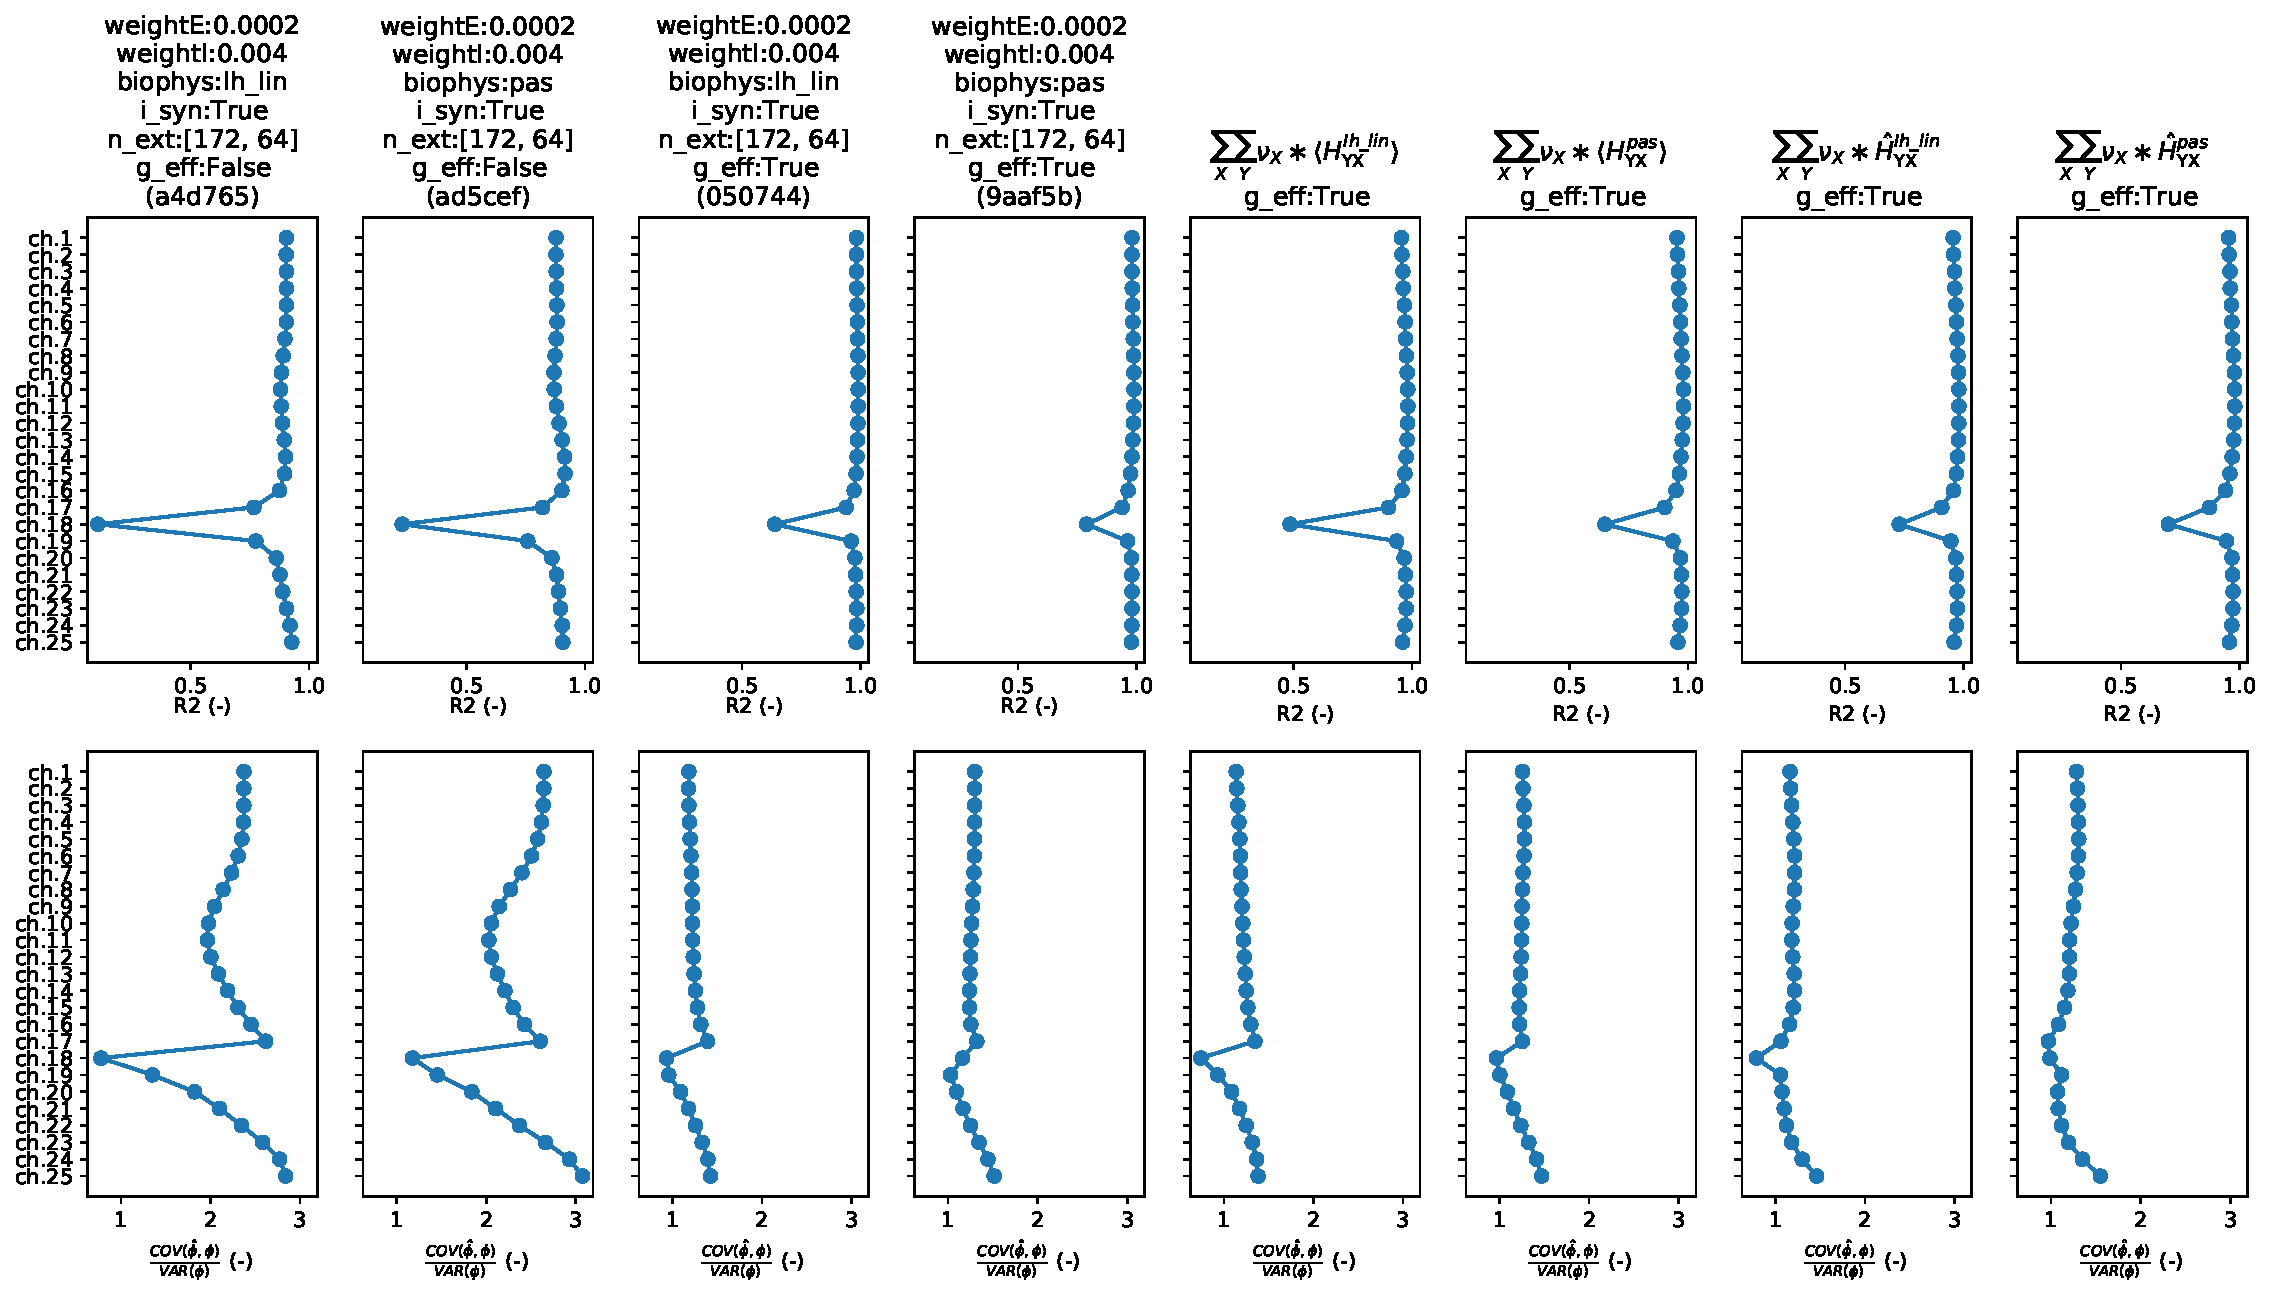
\includegraphics[width=\textwidth]{Figures/Ch-LFPy/Ch-LFPy-correlations.pdf}
\end{center}
\caption{\textbf{Accuracy of signal predictions vs. ground truth.}
For each approximation shown in \Fref{fig:LFPy_predictions},
their accuracy is evaluated in terms of the Pearson correlation coefficient between approximation and ground truth ($CC(\hat{\phi}, \phi)$, top row) and
their covariance normalized by ground truth signal variance ($COV(\hat{\phi}, \phi)/VAR(\phi)$, bottom row).
}
\label{fig:LFPy_correlations}
\end{figure}



\section{Filter (kernel) based prediction methods}
\ghnote{Kan det her gis en kjapp intro til hva vi skal gjennom. Har ikke full oversikt selv her, men handler dette om at vi kan finne en lineaer mapping fra spike times til $V_e$, og at vi enten (A) kan faa spike times fra punktnevronmodell (Step 1 over), eller, som vi skal vise lenger nede her, fra firing rate models?}

\subsection{Spiking point-neuron network models}
\label{sec:Schemes:KernelLFPy}

The cable equation describing the membrane voltage dynamics across different neuron sections is by definition a linear partial differential equation.
Points 1--5 above \ghnote{In the last of the enumerated lists above? Hadde vaert fordelaktig aa kunne referere mer direkte til den siste lista.} allows for computing a \emph{linear} relation between spikes of each presynaptic neurons and resulting contribution to the extracellular signal(s),
as every component including synaptic conductances and voltage-gated ion channels of this hybridized simulation scheme is linearized and linearly separable with respect to time and space.
The different effects of transmission delays (or transmission delay distributions),
evoked synaptic currents,
filtering of inputs by dendrites plus quasi-active approximation of active ion channels and
linear forward model
may then be combined into a spatiotemporal filter kernel $H_{vu}(\mathbf{r},\tau)$ where $\tau$ denote time lag relative to presynaptic spike times in $s_u(t)$ \cite**{Hagen2016}, 
where $u$ and $v$ denote pre- and postsynaptic neuron indices, respectively.
One may compute this filter as
\begin{equation}
H_{vu}(\mathbf{r},\tau) \coloneq \mathbf{F}^{\langle j \rangle} \left[ \overline{I}_{\mathrm{syn}YX} \left( \delta(t - \Delta_{vu} \ast f_{YX} \ast G_{vu} \right)(\mathbf{r}, \tau) \right]~,
\end{equation}
where the Green's like functions $G_{vu}(\mathbf{r}, \tau)$ encompass all dendritic filtering effects on the synaptic input currents into each corresponding distribution of transmembrane currents $\mathbf{I}_\mathrm{m}^{\langle ij \rangle}(\mathbf{r}, \tau)$.
If each kernel function which is specific to each pair of pre- and postsynaptic neuron can be computed,
one could compute the signal as the sum over convolutions between presynaptic spike times and corresponding kernels as
\begin{equation}
\phi(\mathbf{r}, t) = \sum_X \sum_Y \sum_{u \in X} \sum_{v \subset Y} \left(s_u \ast H_{vu} \right)(\mathbf{r}, t)~.
\end{equation}
In large networks however,
computing the full set $H_{vu}(\mathbf{r},\tau)$ can become intractable as the number of connections $K_{YX}$ (and consequently the number of kernels) grow proportionally to the product $N_X N_Y$ if the connection probabilities are kept fixed.
However, \citeasnoun**{Hagen2016} showed that a good approximation to the signal $\phi(\mathbf{r}, t)$ could be obtained by estimating kernels averaged over all pre- and postsynaptic neurons in each population $X$ and $Y$. These averaged kernels may be defined as
\begin{equation}
\langle H_{YX} (\mathbf{r}, \tau) \rangle = \frac{1}{N_X} \sum_{u \in X} \sum_{j \subset Y} H_{vu}(\mathbf{r}, \tau)~.
\end{equation}
In order to compute these kernels averaged directly,
actual network spiking activity may first be replaced by simultaneous and deterministic events
$s_u(t) = \delta(t - t_X)$ where $t_X > 0$ is a chosen time for each population $X$,
compute via the disassociated network model the signal contributions of each postsynaptic population $\phi_{YX}(\mathbf{r}, t)$ around $t_X$
and average the response as
\begin{equation}
\langle H_{YX} (\mathbf{r}, \tau) \rangle = \frac{1}{N_X} \phi_{YX} (\mathbf{r}, \tau)
\end{equation}
where $\tau$ denote time relative to $t_X$.
It is worth mentioning that these kernels are causal, that is,
by construction $\langle H_{YX}(\mathbf{r}, \tau) \rangle \coloneq 0$ for $\tau < 0$ as any contribution to the signal $\phi(\mathbf{r}, t)$ is solely postsynaptic which in this scenario can not occur before the presynaptic spike event at $\tau=0$.
The time lags spanned by the kernels are also symmetric around $\tau=0$ and of finite duration --
the postsynaptic responses typically decay to approximately zero after a few tens of milliseconds.
This decay time is related to the time constants relevant to the neuronal dynamics (that is, $\tau_\mathrm{m}, \tau_\mathrm{syn}, \tau_\mathrm{w}, \ldots$).  
In \Fref{fig:LFPy_kernels} we show a set of such kernels for the stylized two-population multicompartment neuron network illustrated in \Fref{fig:LFPy_network}, 
computed with either quasi-active or fully passive membrane dynamics. 



Finally, if we define the presynaptic population spiking activity as the sequence of Dirac delta distributions $s_X(t) \coloneq \sum_{u \in X} s_u(t)$,
the final signal approximation $\hat{\phi}(\mathbf{r}, t) \approx \phi(\mathbf{r}, t)$ may then be computed as the sum over convolutions
\begin{equation}
\hat{\phi}(\mathbf{r}, t) = \sum_X \sum_Y \left(s_X \ast \langle H_{YX} \rangle \right)(\mathbf{r}, t)~.
\end{equation}

A valid implementation alternative to the linear convolutions showcased here is applying the kernels using a linear filter function implementation.
The measured kernels are essentially finite impulse responses (FIR) that must be 0 for all time lags $\tau < \Delta t$.
\ehnote{The assumed symmetry around $\tau=0$ assumes application of the kernels using a convolution operation. 
The kernel coefficients can also be applied as a (in)finite impulse response (IIR/FIR) function using a standard linear filter implementation such as scipy.signal.lfilter by discarding coefficients for $\tau < 0$ in the IIR case, 
and $\tau <= 0$ in the FIR case.}


\subsubsection{\blue{Population firing rate models}}
\label{sec:Schemes:populationmodels}
\index{Firing rate model}
Similar to how \ghtxt{spiking} dynamics of large-scale multicompartment neuron networks \ghtxt{\sout{as reflected by spikes of the individual neurons}} can sometimes be preserved in \ghtxt{\sout{equivalent}simplified} networks of few-compartment or spiking point neurons \ghtxt{\sout{after a series of simplifying steps}}, further successive steps of simplification may be applied to point-neuron networks in order to describe neuronal dynamics at the level of populations. Such models are commonly referred to as \emph{rate models} as an umbrella term, and may explain a host of observed phenomena on the \emph{mesoscopic} (local populations, brain areas) and \emph{macroscopic} (whole brain) level such as oscillations.


\ghtxt{\sout{Rate models may simply describe the mean activity of subsets of neurons (`populations') as function of time but may also explain activity both in space and time.} The simplest rate models describe the mean activity of subsets of neurons (`populations') as function of time alone, but other versions exist that describe activity both in space and time. } The latter is sometimes referred to as \emph{neural fields} and may readily produce observed phenomena such as traveling waves of activity (see e.g., \cite**{Amari1977,Deco2008}). Certain rate model frameworks may also describe activity of individual neurons. Here, we will however not delve into much mathematical detail as the body of literature on both rate models and neural fields and their derivation is vast, see for example \cite**{Gerstner2014} and \cite**{Ermentrout2010}. As an example, we will merely show that in their simplest form the activity $A(t)$ in a rate model may be described by (Equation 15.17 in \cite**{Gerstner2014})
\begin{equation}
\tau_\mathrm{m} \frac{\partial A(t)}{\partial t} = - A(t) + g_\sigma( I(t) ) ~,
\end{equation}
where $\tau_\mathrm{m}$ is the time constant of the effective low pass filter characterizing the system, $I(t)$ describes the input current (from external and recurrent sources) and $g_\sigma$ a stationary gain function (see \cite**{Gerstner2014} for details).
\ehnote{mulig jeg kan gaa inn i bittelitt mer detalj her og bruke likning 15.18-19 fra seksjon 15.3.2 som eksempel her i stedet}


What we will primarily focus on here,
is how the hybrid forward modeling scheme and the above `kernel trick' idea may be adapted for use with population rate models in a consistent manner.
Let us first make a series of assumptions:
\begin{enumerate}
\item The rate model accurately captures the fluctuations in spike rate of different populations of recurrently connected network of point neurons.
As before, the point-neuron network \textit{may} even have been derived by systematic reduction of detail in a biophysically detailed multicompartment neuron network.
We do not make that a strict requirement however,
as many rate models are phenomenological or have had their parameters determined by parameter fitting to either experimental or model data.

\item The rate model framework allows for specifying key neuron and connectivity parameters such as
population sizes ($N_X, N_Y$) average synaptic in-degree ($\langle k_{YX} \rangle$) or connection probabilities $C_{YX}$,
synaptic coupling strength ($\overline{I}_{\mathrm{syn}YX}$),
synaptic temporal kernel ($f_{YX}(t)$) and
conduction delay distribution $\widetilde{\Delta}_{YX}(t)$ for each connection.
Let us for now assume that these parameters are used to derive parameters and variables entering the actual rate equations (such as $\tau_m, g_\sigma$).
If that is not the case, the magnitude and physical unit(s) of the final signal predictions may be arbitrary and dimensionless, respectively.

\item We let the continuous variable $\nu_X(t)$ describe the population-averaged firing rate (with unit spikes \si{\per\second}) for all $N_X$ neurons in each population $X$ as predicted by the rate model.
\ehnote{legg til "spikes" som enhet til SI pakka}
Conceptually this quantity is equivalent to the discrete population spike signal $s_X(t)$ convolved with some normalized temporal filter kernel or windowing function $f_\mathrm{w}(\tau)$, that is:
\begin{eqnarray}
\nu_X(t) &\equiv& \frac{1}{N_X} \left(s_X \ast f_w \right)(t)~\text{, where} \\
\int_{-\infty}^\infty f_\mathrm{w}(\tau) d\tau &=& 1 ~.
\end{eqnarray}
Choices for filter $w$ could be (but is not limited to) a boxcar, Gaussian or Hamming type windowing function which is symmetric around $\tau = 0$.

\end{enumerate}

Granted that we already computed population-averaged spatiotemporal kernels $\langle H_{YX} (\mathbf{r}, \tau) \rangle$ for the particular pre and postsynaptic network populations ($X, Y \subseteq X$) our rate model represents as above,
we could persevere and compute our signal as
\begin{equation}
\phi(\mathbf{r}, t) = \sum_X N_X \sum_Y \left( \nu_X \ast \langle H_{YX} \rangle \right)(\mathbf{r}, t) ~.
\end{equation}
However, such an approach implies that we must first perform a series of very computationally demanding calculations
in order to compute transfer functions averaged over many thousands of multicompartment neurons.
Can we deduce a methodology to compute a set of deterministic kernels $\hat{H}_{YX}(\mathbf{r}, \tau)$ we need for all pre- and postsynaptic populations $X$ and $Y$ directly,
based on some expectation values for cell and synaptic placements?
Let's try!
First, let us assume that:
\begin{enumerate}
\item The mean synaptic input to every `neuron' in each population is the same.
Thus we may assume that each postsynaptic population can be represented by \emph{one} typical biophysically detailed neuron model. 
In \Fref{fig:LFPy_kernel_predictor}{\bf A} we show geometries used for each population $E$ and $I$ in relation to points in space where extracellular potentials are computed. 
Panel {\bf B} shows the assumed spatial distribution of somas along the vertical $z$-axis. 
The somas are assumed to be placed with homogeneous density within a radius $R$ in the horizontal $xy-$plane (not shown).
We can define the distribution of somas in space as the probability density function $\widetilde{\mathbf{r}}_X$ introduced earlier. 
 
\item Further we assume that the statistics of synaptic placements and currents would be preserved,
which allows us to compute the average synaptic current density for each recurrent connection over the whole postsynaptic `neuron'.  
%which fulfills
%\begin{equation}
%\iiint_{\Omega_\mathrm{syn}} \rho_{\mathrm{syn}YX}(\mathbf{r}, \tau) d\Omega_\mathrm{syn} = k_{YX} \overline{I}_{\mathrm{syn}YX} f_{YX}(\tau) ~.
%\end{equation}
%Here, $\Omega_\mathrm{syn}$ denotes the synaptic input domain, that is, the neuron  membrane hence the unit of $\rho_{\mathrm{syn}YX}(\mathbf{r}, \tau)$ is proportional to \si{\ampere\per\metre^2}.
%(One \emph{could} also define this quantity per unit length.)
%\ehnote{skriv om! Trenger ikke $\rho_{\mathrm{syn}YX}$}

%\item $\rho_{\mathrm{syn}YX}(\mathbf{r}, \tau)$ 
\item Synaptic placements depends on some spatial specificity of synaptic connections \( \mathcal{L}_{YXL}(\mathbf{r}) \) and areas of putative target sections.
If we for instance only allow synaptic input within a certain depth interval $[z_1, z_2]$ where $z_1 < z_2$ (e.g., corresponding to the thickness of a cortical layer),
this spatial specificity function may be defined as
\begin{equation}
\mathcal{L}_{YXL}(z) = \Theta(z - z_2) - \Theta(z - z_1) ~,
\end{equation}
where $\Theta(z)$ denotes the Heaviside step function. 
Alternatively, one could assume normal-distributed synaptic placements, that is, 
$\mathcal{L}_{YXL}(z)\propto \mathcal{\widetilde{N}}(\langle z \rangle, \sigma_z)$ 
around some mean depth $\langle z \rangle$ with standard deviation $\sigma_z$.

\item Furthermore, we let the synaptic density be proportional to the membrane area of postsynaptic compartments $\mathbf{A}_Y$ weighted by $\mathcal{L}_{YXL}$.
Hence the expectation value for synaptic in-degree per compartment indexed by $w$ can be defined as
\begin{equation}
\langle k_{\mathrm{syn}YXw} \rangle \coloneq \frac{K_{YX}}{N_Y} \frac{ \mathcal{L}_{YXL}(z_w) \mathbf{A}_{Yw}}{\sum_w \mathcal{L}_{YXL}(z_w) \mathbf{A}_{Yw}} ~,
\end{equation}
where $z_w$ denotes the center location of each compartment projected on the $z$-axis.
With this quantity one may define the transfer function  of firing rate of population $X$ to each per-compartment synaptic input current as
\begin{equation}
H_{\mathrm{syn}YXw}(\tau) = N_X \langle k_{\mathrm{syn}YXw} \rangle \overline{I}_{\mathrm{syn}YX} \left( \widetilde{\Delta}_{YX} \ast f_{YX}\right)(\tau) ~.
\end{equation}

\item We will assume that the the linearization tricks applied to the membrane of neuron models representative of each population remain valid for rate-based frameworks,
meaning we allow for purely passive or quasi-active membrane descriptions.
Then one may straightforwardly compute the resulting postsynaptic response
(i.e., $\mathbf{I}_\mathrm{m}(\mathbf{r}, \tau),{}\mathbf{I}_\mathrm{a}(\mathbf{r}, \tau))$
by applying synaptic currents of $H_{\mathrm{syn}YX}(\tau)$ in a single multicompartment neuron simulation for connections between populations $X$ and $Y$.

\item One could now compute each rate-signal transfer function or kernel from the current distribution
$\mathbf{I} \in \{ \mathbf{I}_\mathrm{m}(\mathbf{r}, \tau), \mathbf{I}_\mathrm{a}(\mathbf{r}, \tau) \}$ as
\begin{equation}
\hat{H}_{YX}(\mathbf{r}, \tau) = \mathbf{F}\mathbf{I}(\mathbf{r}, \tau) ~,
\end{equation}
however, this would would imply that the cell-body distribution in each postsynaptic population would be condensed to a point $\delta(\mathbf{r} - \mathbf{r}_Y)$.
Assuming that the $N_Y$ cell bodies are sampled from the distribution $\widetilde{\mathbf{r}}_Y$
(recall our initial description of the biophysically detailed network model in \Fref{chap:LFPy:hybrid}),
one could consider computing an equivalent volumetric current field by convolving the predicted currents $\mathbf{I}(\mathbf{r}, \tau)$ with the normalized spatial function
$\widetilde{\mathbf{r}}_Y / \iiint_\Omega \widetilde{\mathbf{r}}_Y d\Omega$
and then compute and apply the forward solution $\mathbf{F}$.
A more straightforward and equivalent alternative, however,
is simply to embed the spatial averaging in the mapping matrix $\mathbf{F}$ directly.
In case of the point source formula for extracellular potentials its elements of can be computed as
\begin{equation}
f_{ij} = \frac{1}{4 \pi \sigma \iiint_\Omega \widetilde{\mathbf{r}}_Y d\Omega}
	\iiint_\Omega \frac{d\Omega}{\Vert \mathbf{R}_i - \mathbf{r}_j - \mathbf{r}_\Omega \Vert}~, 
\end{equation}
where points $\mathbf{r}_\Omega \sim \widetilde{\mathbf{r}}_Y$. 
Analytical solutions are however only possible to derive for certain source geometries, 
hence numerical integration methods will usually be required. 
Our assumption of point sources in this context in contrast to line sources is motivated by the fact that the typical segment extents are small compared to the extent of $\widetilde{\mathbf{r}}_Y$.

\end{enumerate}


\section{Intermezzo: Quantitative comparison of predictions using hybrid scheme and rate predictor}
\label{sec:Schemes:comparison}
\ghnote{Jeg synes dette er fint og orienterende. Er det en tanke aa ha noe ala dette tidlig i kapittelet, som en slags introduksjon til det vi skal pine oss igjennom av teknikaliteter? Kan det lages et slags diagram over mulighetene. Step 1: Regne ut spike times eller rates (punktnevroner vs ratemodeller). Step 2: Mate dem inn i MC-modeller av ulik kompleksistet. Step 3: Regne ut LFP med VC teori. Step 2-3 kan erstattes med en filter-kernel som mapper Step 1 direkte til Step 3. Her oppstaar soet musikk og god overensstemmelse som vist i noen av disse pene figurene. Under skal vi gaa gjennom hele treskeriet som maa til for aa oppnaa denne soete musikken.... etc.}

Before considering other approximate schemes for predicting extracellular signals of interest, 
we shall briefly compare predictions using the `hybrid scheme' (\Fref{sec:Schemes:HybridLFPy}),
averaged hybrid scheme kernels (\Fref{sec:Schemes:KernelLFPy}),
and the deterministic population firing rate kernel predictor (\Fref{sec:Schemes:populationmodels}) to the ground truth signal predictions of the recurrent multicompartment neuron network model. 

The full network model constructed from two populations of active, stylized multicompartment neuron models and resulting activity is summarized in \Fref{fig:LFPy_network}. 
The main basis of comparison is the `real' ground truth extracellular potential shown in panel E. 
Together with the actual network specification (geometry, connectivity, cell properties), 
the hybrid scheme mainly takes the spiking activity (panel C) as its input. 
The kernel-based approximations utilize the corresponding firing rates (panel D). 

For the hybrid scheme, 
we will consider four different cases, that is, using quasi-active neuron models (`biophys:Ih\_lin') or fully passive (`biophys:pas') neuron models, 
and ignore (`g\_eff:False') or account (`g\_eff:True') for changes to the effective membrane time constants resulting from synaptic conductances.  
Comparing the extracellular potentials across depth in \Fref{fig:LFPy_predictions},
it becomes immediately evident that predictions that do not account for changes in effective membrane time constants (columns 2 and 3) overestimate the typical signal amplitudes of the real signal, 
irrespective of the choice of linear membrane model. 
By visual inspection, the converse predictions utilizing an effectively reduced membrane time constant (columns 4 and 5) preserve both the signal amplitudes across channels and temporal dynamics of the ground-truth signal. 
This excellent agreement is quite surprising as the hybrid-scheme predictions do not account for any signal contributions by action potentials. 
Note however, that this observation can be explained by the fairly low on average per-neuron firing rates (cf. \Fref{fig:LFPy_network}C) which means that synaptic contributions govern the extracellular potentials.

For signal predictions set up either using spatiotemporal filter kernels for each recurrent connection from the hybrid scheme ($\langle H_{YX}(\mathbf{r}, \tau) \rangle$ in \Fref{fig:LFPy_kernels}) or deterministic rate-model version  ($\hat{H}_{YX}(\mathbf{r}, \tau)$ in \Fref{fig:LFPy_kernel_predictor}), 
the final signal approximations shown in \Fref{fig:LFPy_predictions} columns 6-9 is virtually identical to the hybrid scheme predictions. 
\Fref{fig:LFPy_correlations} compares across all channels both the Pearson correlation coefficients $CC(\hat{\phi}, \phi)$ between each approximation $\hat{\phi}$ and ground truth signal $\phi$ as well as covariance normalized by variance $COV(\hat{\phi}, \phi)/VAR(\phi)$. 
In all respects, the hybrid scheme with effective membrane time constants as well as the different kernel predictions demonstrate excellent agreement with the ground truth, except for channel 18 which is subject to the lowest overall signal amplitude (due to local cancellation effects). 
Otherwise $CC(\hat{\phi}, \phi) \lesssim 1$ which imply near perfect temporal agreements, 
while the normalized covariance measure $COV(\hat{\phi}, \phi)/VAR(\phi) \gtrsim 1$ imply that the steps that were incorporated did not introduce some arbitrary scaling factor in the approximated signals. 
The choice of cable model, that is, quasi-active linear or passive linear, has minor impact on the different predictions.   


\section{\blue{EH: Other approximations}}
\label{sec:Schemes:proxies}

So far, we have showed by example that linearized computational schemes can well explain the extracellular potentials (and by extension magnetic signals) from recurrently connected networks of multicompartment neuron models. 
These linear approximations were all derived from the recurrent network specification itself. 
In order to predict signals from point-neuron networks or rate models however, 
various assumptions on the anatomy of the neurons, connections etc. must be incorporated, 
which is made difficult by the fact that such anatomical data from experiments are generally lacking. 
For the purpose of relating in particular point-neuron network activity to extracellular electric or magnetic measures of activity,
a number of heuristic signal approximations (``proxies'') have still been proposed and utilized in the literature. 
These proxies are, however, for the most part poorly grounded in the biophysics of extracellular electric and magnetic signals. 

Using a computational model setup reminiscent of the hybrid scheme applied to a cortical microcircuit model in \cite**{Hagen2016} outlined throughout \Fref{sec:Schemes:HybridLFPy},   
\cite**{Mazzoni2015} compared different LFP proxies that could be extracted in two-population spiking point-neuron network models. 
These proxies, where some have been used to mimic the LFP, EEG or similar in past studies, 
were by \cite**{Mazzoni2015} defined as the convolution between linearly separable components as
\begin{equation}
\phi_\text{proxy}(\mathbf{r}, t) = f_\text{proxy}(\mathbf{r}) \ast g_\text{proxy}(t)~, 
\end{equation}
where the spatial function $f_\text{proxy}(\mathbf{r})$ defines the overall signal variance and sign, 
and $g_\text{proxy}(t)$ a position-independent temporal component. 
By construction, the temporal component has zero mean and variance of unity. 
As a ground truth extracellular potential signal $\phi(\mathbf{r}, t)$ was computed, 
different choices of $g_\text{proxy}(t)$ could be evaluated while fitting the corresponding spatial functions $f_\text{proxy}(\mathbf{r})$. 
The ground truth LFP signal was predicted using the standard MC formalism in combination with the line-source volume conductor model.
Synaptic activation times were determined by the spiking activity of a two-population point-neuron network model  with current-based synapses taken from a previous study \cite**{Cavallari2014}. 
The LFP signal was also computed at different depths and lateral offsets, 
mimicking an experimental recording using a laminar probe inserted down through a cortical column. 
Hence, performance of the different proxies could be evaluated across different depths. 

So which choices for $g_\text{proxy}(t)$ can be considered? 
In spiking point-neuron networks one can with relative ease record events and compute 
the population-averaged spike rates $\nu_X(t)$ for each population $X$, 
the population-averaged voltages $\langle V_X(t) \rangle$ of the point neurons
and the summed synaptic currents resolved into excitatory (AMPA) and inhibitory (GABA) contributions onto different subpopulations.
Then one can also consider linear combinations of the synaptic currents. 
%the absolute of the summed synaptic currents amounting to the difference between them (as their sign is opposite), 
%and finally a weighted sum of the mean-subtracted summed synaptic currents with added delays along the time axis.

The task at hand was identifying which proxy maximises the fraction of variance explained ($R^2$) between the  ground-truth LFP signal and the respective proxy predictions. 

As expected, both the population firing rate proxy ($\sum_X \nu_X(t)$) performed poorly as it can not possibly account for any spatial or temporal filtering effects mediated by the actual spike-signal kernel functions $H_{YX}(\mathbf{r}, \tau)$. 
While the somatic voltage proxy account for conduction delays and
temporal components of synaptic currents but without intrinsic dendritic filtering, 
its performance is only marginally better as the signals in question reflect transmembrane currents which do not equate fluctuations the membrane voltages. 
That leaves the various linear combinations of excitatory and inhibitory synaptic input currents, 
which \textit{a priori} ignore additional linear contributions by intrinsic dendritic filtering and the electrostatic forward model in question. 
Using the nomenclature established throughout this Chapter, 
these temporal components $g_\text{proxy}(t)$ of the proxy LFPs can be defined as \cite**{Mazzoni2015}:
%
\begin{eqnarray}
z_\text{score}\left(u(t)\right) &=& \frac{u(t)-\mu_u}{\sigma_u} \\
g_{\sum I_E}(t) &=& z_\text{score} \bigg( \sum_{X=E} \sum_{Y=E} K_{YX} \big( \nu_X \ast \widetilde{\Delta}_{YX} \ast I_{\text{syn}YX})(t) \bigg) \\
g_{\sum I_I}(t) &=& z_\text{score} \bigg( \sum_{X=I} \sum_{Y=E} K_{YX} \big( \nu_X \ast \widetilde{\Delta}_{YX} \ast I_{\text{syn}YX})(t) \bigg) \\
g_{\sum I}(t) &=& z_\text{score}\bigg( \sum_X \sum_{Y=E} K_{YX} \big( \nu_X \ast \widetilde{\Delta}_{YX} \ast I_{\text{syn}YX})(t) \bigg) \\
g_{\sum {|I|}}(t) &=& z_\text{score} \bigg(  \sum_X \sum_{Y=E} \big| K_{YX} \big( \nu_X \ast \widetilde{\Delta}_{YX} \ast I_{\text{syn}YX})(t) \big|  \bigg) \\
g_\text{WS}(t) &=& z_\text{score} \bigg(  \sum_X \sum_{Y=E} \big| \alpha_X K_{YX} \big( \nu_X \ast \widetilde{\Delta}_{YX} \ast I_{\text{syn}YX} \ast \delta(t-\tau_X) \big)(t) \big|  \bigg)~. 
\end{eqnarray}
%
Here, the $z$-scoring function ensures temporal components with zero mean and unitary variance. 
For the latter function \textit{weighted sum} temporal component $f_\text{WS}(t)$ the parameter $\alpha_X$ is scalar and for the excitatory connections $\alpha_{X=E} \coloneq 1$,
while the term $\delta(t-\tau_X)$ denotes a temporal delay. 
In conjunction with corresponding spatial weighting functions $f_\text{proxy} (\mathbf{r}) \in \{ f_{\sum {I_I}}, f_{\sum {I_I}}, f_{\sum I}(\mathbf{r}), f_{\sum {|I|}}(\mathbf{r}), f_\text{WS}(\mathbf{r}) \}$ which allows for defining the proxy signal as
\begin{equation}
\phi_\text{proxy}(\mathbf{r}, t) = f_\text{proxy}(\mathbf{r}) \ast g_\text{proxy}(t)~.
\end{equation}
%
In this formalism, the elements of each $f_\text{proxy}(\mathbf{r})$ and free parameters in $g_\mathrm{WS}(t)$ can then be trivially fitted by minimizing the mean squared difference between ground truth signal and proxy signals 
\begin{equation}
\text{MSE}_\text{proxy} = \langle \left(\phi(\mathbf{r}, t) - \phi_\text{proxy}(\mathbf{r}, t)\right)^2 \rangle ~.
\end{equation}
%
For the two-population set up in \cite**{Mazzoni2015} the best-fitting proxy was determined to be the weighted sum variant $\phi_\text{WS}(\mathbf{r}, t)$ with parameters entering the temporal component set as $\tau_\text{E} =~$\SI{6}{\milli\second}, $\tau_\text{I}=0$, $\alpha_\text{E}=1$ and $\alpha_\text{I} = 1.65$, 
resulting in up to $93\%$ variance explained in certain locations $\mathbf{r}$. 

As a proof of principle, we compare these different LFP proxies against the ground truth LFP generated by our recurrently connected multicompartment network model. 
In \Fref{fig:g_proxy}A different temporal components $g_\mathrm{proxy}(t)$ derived similar to \cite**{Mazzoni2015} but from the recurrent multicompartment neuron network are compared. 
The corresponding panel B shows their fraction of variance explained (R2) against the ground truth extracellular potential measured across different depths. 
These results show that the temporal fluctuations in the extracellular potential are very well explained by the summed inhibitory synaptic current onto the excitatory population across most channels. 
The firing rate and excitatory synaptic currents shows the worst agreement,  
however, panel C shows that improved agreements in terms of R2 can be achieved by applying a temporal shift to the respective components. 
Dependent on on location, 
either the inhibitory synapse current or absolute sum of synaptic currents maximize proxy performance 
-- thus for the sake of simplicity inhibitory synapse currents could well provide a valid indication of the temporal properties of extracellular measurements of activity from simplified neuronal network models. 


\begin{figure}[!ht]
\begin{center}
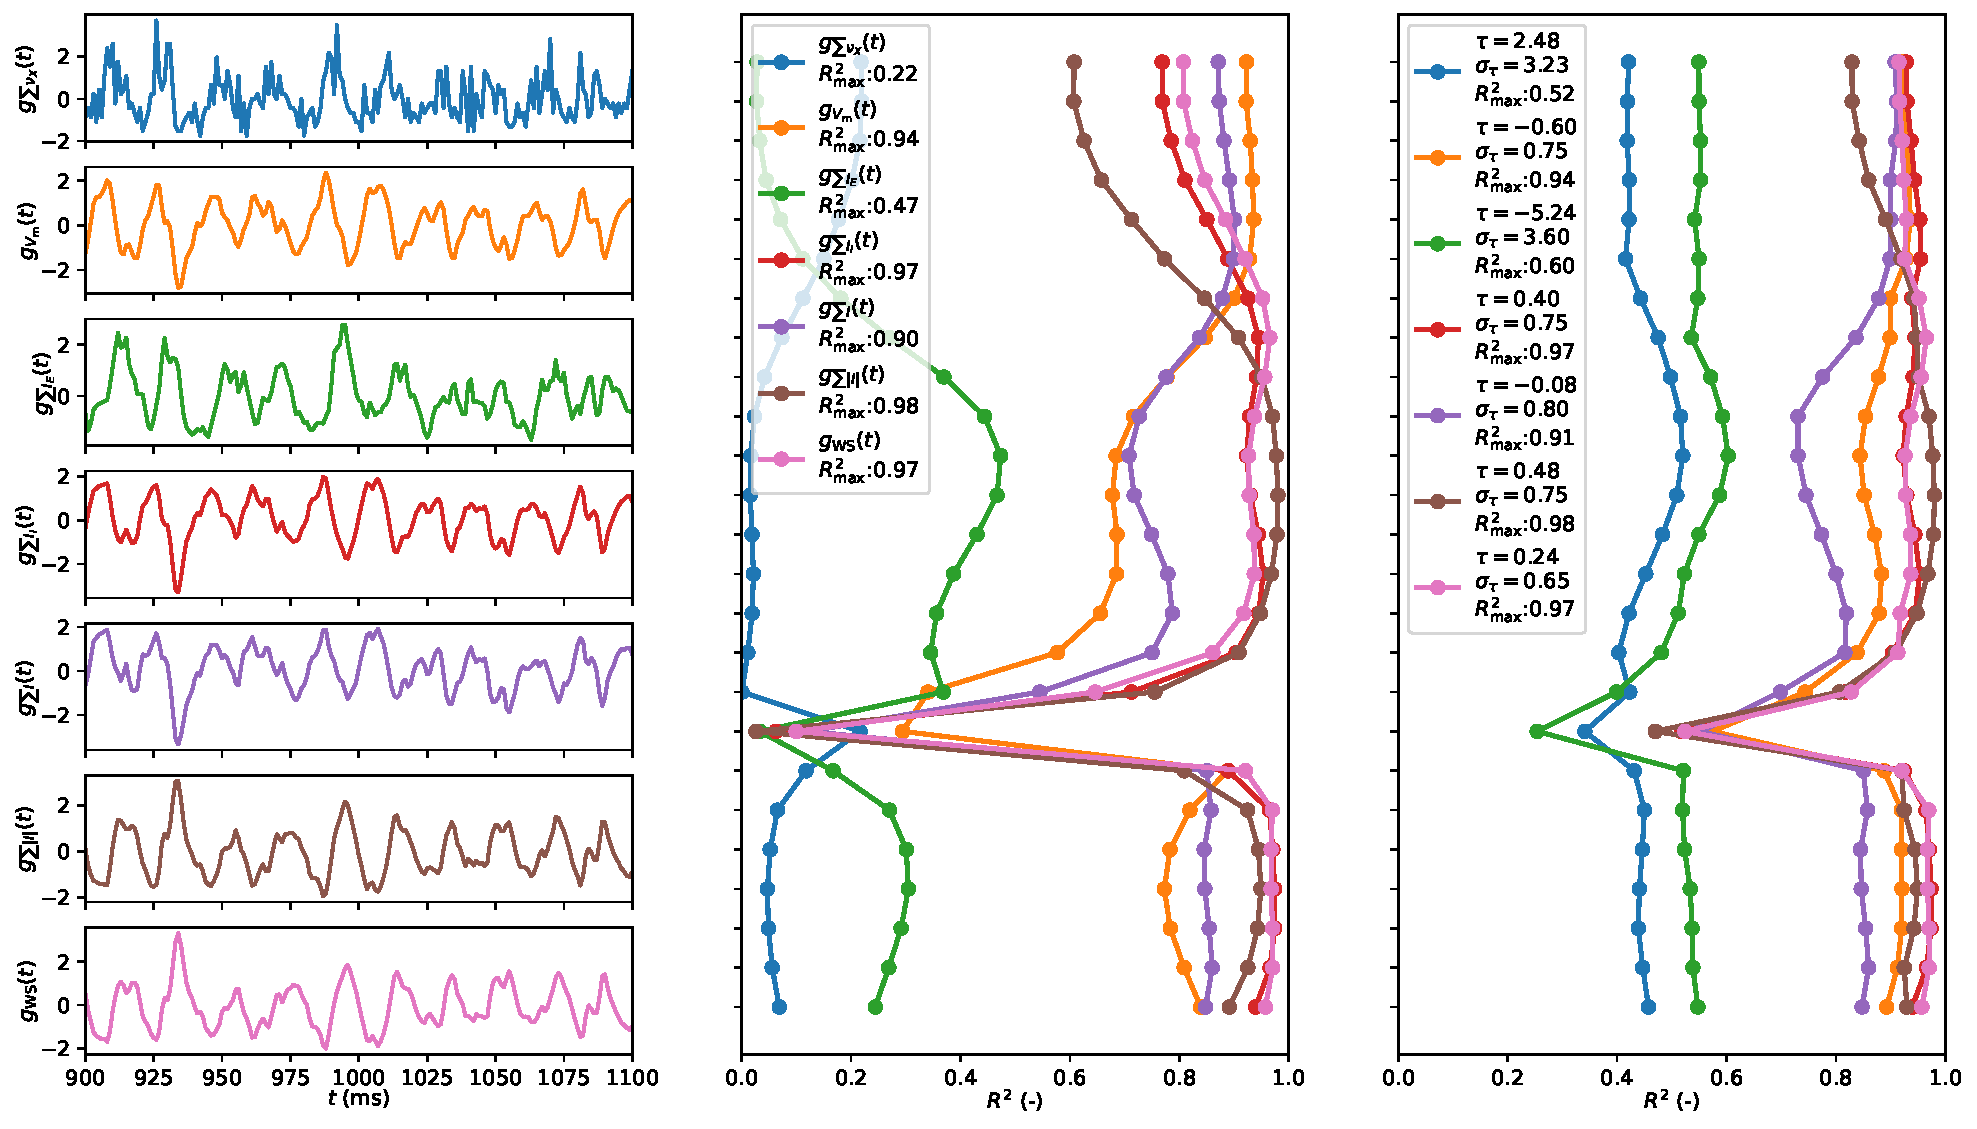
\includegraphics[width=\textwidth]{Figures/Ch-LFPy/Ch-LFPy-g_proxy.pdf}
\end{center}
\caption{\textbf{Comparison of temporal proxy components $g_\mathrm{proxy}(t)$.} 
{\bf A} Snapshots of normalized temporal components of different candidate proxy signals for mimicking extracellular signals from recurrent network model. 
{\bf B} Ratio of variance (R2) explained by the different temporal components across channels without time shifts. 
{\bf C} Same as panel B but for temporal delay values $\tau$ which maximizes R2 in each individual channel. 
The legend shows the corresponding mean and standard deviation of the delays.
\ehnote{todo: WS. Veit ikke om det er saa fryktelig viktig aa vise kurver for $f_{proxy}$ her.} 
}
\label{fig:g_proxy}
\end{figure}

